\chapter{Оценки тензорных рангов и явные QTT-разложения для матриц, обратных к  некоторым циркулянтным}\label{ch:ch1}


%\maketitle
%\begin{abstract}
%	%In this paper, we are concerned with the inversion of circulant matrices, their quantized tensor-train~(QTT) rank bounds and explicit QTT representation.
%	В данной работе мы рассматриваем инверсию циркулянтных матриц и их квантованную структуру тензор-трейн~(QTT).
%	В частности, мы показываем, что обратная комплексная циркулянтная матрица $A$, порожденная первым столбцом вида $(a_0,\dots,a_{m-1},0,\dots,0,a_{-n},\dots, a_{-1})^\top$, допускает представление QTT с рангами QTT, ограниченными $(m+n)$.
%	При определенных предположениях на записи $A$ мы также получаем явное QTT-представление $A^{-1}$. Последнее может быть использовано, например, для преодоления проблем устойчивости, возникающих при численном решении дифференциальных уравнений с периодическими граничными условиями в формате QTT.
%\end{abstract}
% 	\section{Plans and ideas}
% 	\begin{enumerate}
% 		\item Proof of case of $[a_0, \dots, a_{n-1}, 0, \dots]$
% 		\item Proof of case of $[a_0, \dots, a_{m-1}, 0, \dots, 0, a_{-q}, \dots, a_{-1}]$
% 		\item Does it follows from the invertibility of $A$ that the polynomials don't have roots on the unit circle?
% 		\item Check both cases numerically. Done: \url{https://colab.research.google.com/drive/103BVBb9LBtD5oCCVqK0eUeYkc_zbf4O-?usp=sharing}
% 		\item Explicit formulas for cases of mass matrix, stiffness matrix and Laplace operator matrix (see pdf-s with whiteboards) [are these their real names ???]
% 		\item Two-level circulants
% 		\item How many simple roots do polynomials actually have inside the unit circle?
% 		Check for random polynomials and some interesting concrete ones (which ones ???) 
% 		\textbf{Seems it doesn't matter}: rank is equal to the number of roots of $g(z)$ inside the unit circle plus number of roots of $g(z^{-1})$ inside the unit circle, i.e. $\deg g(z)$.
% 		\item Close roots give low-rank approximations.
% 		\item We can fill the unit circle uniformly with points and thus get a low-rank approximation to any inverse circulant (?!!) 
% 	\end{enumerate}
%     \newpage	
\section{Введение}

Тензорно-тензорное (ТТ) разложение~\cite{osel-tt-2011} - это нелинейное представление многомерных массивов (тензоров), которое во многих случаях приводит к значительным коэффициентам сжатия при сохранении высокой точности аппроксимации.
Примечательно, что TT также может применяться к низкоразмерным данным.
Например, вектор (одномерный массив) из $\mathbb{C}^{2^\LL}$ может быть переформирован в элемент $\mathbb{C}^{2 \times \dots \times 2}$ ($\LL$-мерный тензор), и тогда становится применимым TT-разложение.
Эта идея была предложена в ~\cite{osel-2d2d-2010,khor-qtt-2011} и известна под названием квантованного TT (QTT) разложения.
Разложение QTT оказалось полезным в различных приложениях, в частности, для аппроксимации функций и решения дифференциальных уравнений (PDE)~\cite{khoromskij2018tensor}.

Разложение QTT также может быть применено к линейным операторам в виде матриц.
Это необходимо для построения решателей линейных систем, когда правая часть задана в формате QTT, а цель состоит в аппроксимации решения также в формате QTT с желаемой точностью.
В данной работе мы заинтересованы в изучении QTT-представления обратной полосы циркулянтной матрицы:
\begin{equation}\label{eq:A}
A=
\begin{bmatrix}
a_0     & a_{-1} & \dots  & a_{-n} & 0      & \dots  & 0       & a_{m-1} & \dots  & a_1     \\
a_1     & \ddots &        &        & \ddots &        &         &         & \ddots & \vdots  \\
\vdots  &        & \ddots &        &        & \ddots &         &         &        & a_{m-1} \\
a_{m-1} &        &        & \ddots &        &        & \ddots  &         &        & 0       \\
0       & \ddots &        &        & \ddots &        &         & \ddots  &        & \vdots  \\
\vdots  &        & \ddots &        &        & \ddots &         &         & \ddots & 0       \\
0       &        &        & \ddots &        &        & \ddots  &         &        & a_{-n}  \\
a_{-n}  &        &        &        & \ddots &        &         & \ddots  &        & \vdots  \\
\vdots  & \ddots &        &        &        & \ddots &         &         & \ddots & a_{-1}  \\
a_{-1}  & \dots  & a_{-n} & 0      & \dots  & 0      & a_{m-1} & \dots   & a_1    & a_0    
\end{bmatrix}\in\mathbb{C}^{N\times N},
\end{equation}
который мы также обозначим как $A = \mathsf{circ}(a_0,\dots, a_{m-1}, 0,\dots, 0, a_{-n},\dots, a_{-1})$.
Мы заинтересованы в получении точных ранговых границ QTT для $A^{-1}$ и его явного QTT-представления при $N = 2^\LL$.
Мы подчеркиваем тот факт, что рассматриваемые QTT ранги матриц \emph{не связаны} со стандартным рангом матрицы и, следовательно, малые QTT ранги не означают, что рассматриваемая матрица сингулярна.
QTT ранговые границы $A^{-1}$ могут быть полезны, например, для получения ранговых границ для решения линейных систем с $A$, а явное QTT представление $A^{-1}$ может быть использовано для построения эффективных решателей.

%\paragraph{QTT decomposition.} 
Чтобы формально представить QTT-разложение матрицы, давайте сначала представим QTT-разложение вектора $x = \{x_i\}_{i=0}^{2^\LL-1}\in\mathbb{C}^{2^\LL}$. %\in\mathbb{R}^{2^\LL}$.
Представим $x$ как многомерный массив $X = \{X_{i_1\dots i_\LL}\}_{i_1,\dots, i_\LL=0}^{1,\dots,1}\in\mathbb{C}^{2\times \dots \times 2}$ следующей биекцией между целым числом $i=0,\dots,2^\LL-1$ и бинарными индексами $\LL$ $(i_1,\dots,i_\LL)$: % binarizing the index $i=1,\dots,2^\LL$ such that% that , i.e. encode it with $\LL$ binary indices $i_k\in\{0, 1\}$, $k=1,\dots,\LL$ such that:
\[
i =\overline{i_\LL \dots i_1} \equiv \sum_{k = 1}^\LL 2^{\LL - k} i_k,
\]
что аналогично двоичному представлению $i$.
Затем мы применяем TT-разложение к $X$:
\[
x_{\overline{i_\LL \dots i_1}} \equiv X_{i_1\dots i_\LL} = \sum_{\alpha_1,\dots,\alpha_{\LL-1}=1}^{r_1,\dots,r_{\LL-1}} G_{i_1 \alpha_1}^{(1)} G_{\alpha_1 i_2 \alpha_2}^{(2)} \dots G_{\alpha_{\LL-2} i_{\LL-1} \alpha_{\LL-1}}^{(\LL-1)} G_{\alpha_{\LL-1} i_\LL}^{(\LL)},
\]
где минимальные значения $r_1,\dots,r_{\LL-1}$ называются TT-рангами.
Обратите внимание, что для хранения так называемых \emph{ядерных тензоров}~$G^{(k)}$, $k=1,\dots,\LL$ требуется $\mathcal{O}(\LL r^2)$ байт (здесь $r=\max_k r_k$), что линейно зависит от $\LL$, если ~$r$ ограничено.
Аналогично, мы вводим QTT-разложение матрицы $B = \{B_{i,j}\}_{i,j=0}^{2^\LL-1} \in\mathbb{C}^{2^\LL\times 2^\LL}$, бинаризируя два индекса: $i =\overline{i_\LL \dots i_1}$, $j =\overline{j_\LL \dots j_1}$ и объединяя $i_k,j_k$ в пары:
\begin{equation}\label{eq:tt_mat}
B_{\overline{i_\LL \dots i_1}, \overline{j_\LL \dots j_1}} = 
\sum_{\alpha_1,\dots,\alpha_{\LL-1}=1}^{r_1,\dots,r_{\LL-1}}
G_{i_1 j_1 \alpha_1}^{(1)} G_{\alpha_1 i_2j_2 \alpha_2}^{(2)} \dots G_{\alpha_{\LL-2} i_{\LL-1}j_{\LL-1} \alpha_{\LL-1}}^{(\LL-1)} G_{\alpha_{\LL-1} i_\LL j_\LL}^{(\LL)},
\end{equation}
что приводит к асимптотически одинаковому количеству байт в тензорах ядра $G^{(k)}$, $k=1,\dots,\LL$: $\mathcal{O}(\LL r^2)$.
В качестве примера можно рассмотреть матрицу тождества $I\in\mathbb{C}^{2^\LL\times 2^\LL}$, элементы которой можно выразить в терминах дельты Кронекера $\delta_{\alpha \beta}$ следующим образом:
\[
I_{\overline{i_\LL \dots i_1}, \overline{j_\LL \dots j_1}} = \delta_{i_1 j_1} \delta_{i_2 j_2} \dots \delta_{i_\LL j_\LL},
\]
т.е. без суммирования. Следовательно, все ранги QTT матрицы тождеств равны $1$, хотя матрица имеет полный ранг.

% Indeed, the QTT decomposition applied to matrices is formulated as follows.
% Consider a matrix $B\in\mathbb{R}^{2^\LL\times 2^\LL}$, with the entries $b_{ij}$.
% First, we binarize the index $i$, i.e. encode it with $\LL$ binary indices $i_k\in\{0, 1\}$, $k=1,\dots,\LL$ such that:
% \[
%     i =\overline{i_\LL \dots i_1} \equiv \sum_{k = 1}^\LL 2^{\LL - k} i_k,
% \]
% and similarly for $j$.
%The matrix $B$ can, therefore, be represented as a multidimensional array $\widetilde B$

%\paragraph{The idea.} 
Чтобы вывести ранговые границы QTT для $B=A^{-1}$, где $A$ - как в ~\eqref{eq:A}, мы покажем, что элементы его первого столбца $b$ имеют вид (Section~\ref{sec:circ}):
\begin{equation}\label{eq:first_col}
b_{i} = \sum_{k=1}^s P_{k} (i) z_k^i,
\end{equation}
где $z_k$ - корни из $g(z)=0$ и $h(z)=0$:
\begin{equation}\label{eq:g-and-h}
g(z) = \sum_{k=-n}^{m-1}a_{k}z^{k+n}, \quad h(z) = \sum_{k=-n}^{m-1}a_{k}z^{m-k-1},
\end{equation}
%    
расположенный внутри $U=\{z:|z|<1\}$, и где $P_k(i)$ - некоторый многочлен от $i$ со степенью меньше кратности $z_k$.
Отметим, что в ~\cite{fuyong2011inverse} были получены те же формулы, но для корней со всеми кратностями, равными $1$, а в, например, ~\cite{searle1979inverting} кратности больше $1$ рассматривались, но только для случая $m=2$, $n=1$.
Чтобы преодолеть эти ограничения, мы обобщили результат на случай произвольной кратности.
Мы накладываем на $A$ только одно ограничение, которое является фундаментальным для предлагаемого подхода: полиномы $g(z)$ и $h(z)$ от~\eqref{eq:g-and-h} не должны иметь корней с абсолютным значением 1, как это бывает для сингулярных матриц (но не только для них).

Структура ~\eqref{eq:first_col} используется для оценки QTT рангов $B = A^{-1}$, которые, как оказалось (раздел ~\ref{sec:qtt_ranks}), ограничены $(m+n)$.
В качестве альтернативы можно вывести QTT-представление $b$ и применить результат из~\cite{khkaz-conv-2013} для создания QTT-представления циркулянтной матрицы по ее первому столбцу в формате QTT.
Тем не менее, мы отмечаем, что такой подход приводит к завышенным значениям ранга QTT для $B$.
Разработанные методы применяются к нескольким примерам циркулянтных матриц (раздел ~\ref{sec:examples}), включая случай псевдоинверсий.
%We also note that the straightforward application of the results from~\cite{khkaz-conv-2013} to the QTT representation of $b$ would lead to overestimated QTT rank values of $B$.

В случае простых корней $z_k$ мы дополнительно выводим явные формулы для QTT-представления~$B$ (раздел~\ref{sec:qtt_repr}).
Наконец, мы проверяем устойчивость наших формул численно (раздел ~\ref{sec:num_exp}) на примере одномерной краевой задачи конвекции-реакции-диффузии с периодическими граничными условиями.
Численные результаты показывают, что мы можем применять предложенные явные формулы для больших значений $L$ без каких-либо проблем с устойчивостью.
Это отличается от наивного применения TT-решателей линейных систем непосредственно к матрице $A$, явно собранной в формате QTT.
%This is by contrast to applying TT solvers such as alternating minimal energy method (AMEn) directly to solve a linear system with $A$ given in the QTT format.

%The idea behind our approach is as follows.
%The derived rank bounds and explicit QTT representation are based on the explicit form of a circulant inverse.
%In particular, it can be shown that 

%The rank bounds and the explicit QTT representation are derived from the fact 

%\subsection{Contributions.}
% Our main contributions are:
% \begin{itemize}
%     \item We generalize circulant inversion formulas from~\cite{todo} to the case when certain polynomials, associated with the first column of a general circulant also admit multiple roots (Section~\ref{todo}).
%     \item We apply results from Section~\ref{todo}, and obtain that the tensor rank of $A^{-1}$ with $A$ of the form~\eqref{eq:A} and $N = N_1 N_2$   is bounded by $(m+n)$ (Section~\ref{todo}).
%     \item We obtain explicit QTT representation of $A^{-1}$ with $A$ being a certain subset of matrices of the form~\eqref{eq:A} and $N = 2^{\LL}$  (Section~\ref{todo}), apply it to several particular matrices arising in PDEs (Section~\ref{todo}) and numerically illustrate the robustness of the proposed formulas (Section~\ref{todo}).
% \end{itemize}

\emph{Связанная работа}. Для QTT-аппроксимации векторов, связанных с функциями, мы упоминаем ~\cite{khor-qtt-2011,dk-qtt-tucker-2013,gras-tenz-2010,vysotsky2021tt}.
Техника получения явных QTT-представлений QTT-матриц была разработана в ~\cite{khkaz-lap-2012} и применена к конкретным матрицам, что привело к дискретизации оператора Лапласиана на равномерной сетке.
В~\cite{khkaz-lap-2012} были также приведены инверсии этих матриц в особых случаях граничных условий Неймана и Дирихле.
В случае матрицы Фурье не существует представления QTT с низким рангом, но матрично-векторное произведение все же может быть эффективно аппроксимировано в формате QTT~\cite{dks-ttfft-2012}.
В работе ~\cite{khkaz-conv-2013} были получены ранговые границы QTT и явные формулы для многоуровневых матриц Тоеплица и циркулянта.
Границы рангов для ленточных тоеплицевых матриц были получены в ~\cite{otz-teninv-2011}.

В работе ~\cite{cor-eccomas-2016,kazeev2018quantized,cor-robqtt-2016pre} было замечено, что прямое применение решателей, основанных на оптимизации TT, к линейным системам, возникающим из PDE с матрицами в формате QTT, приводит к серьезным численным неустойчивостям.
Эта проблема была формализована в~\cite{bachmayr2018stability} и возникает как из-за плохой обусловленности дискретизированных дифференциальных операторов, так и из-за плохой обусловленности самих тензорных представлений.
Для преодоления этих проблем в той же работе было предложено явное QTT-представление BPX-обусловленных систем, которое позже было использовано для многомасштабных и сингулярно возмущенных задач в ~\cite{kazeev2020quantized,marcati2020low}.
В работе ~\cite{rakhuba2021robust} был разработан надежный и эффективный решатель, основанный на неявном методе переменного направления (ADI) и явных формулах инверсии для трехдиагональных матриц Тоеплица.
Этот решатель был применен к трехмерным задачам с собственными значениями типа Шредингера~\cite{marcati2019tensor}.

Насколько нам известно, не было получено ни ранговых границ QTT, ни явных формул QTT ни для инверсий циркульантных матриц общей полосы, ни для их частных случаев, таких как одномерная дискретизация лапласиана с периодическими граничными условиями.

% For examples, the explicit inversion of tridiagonal Toeplitz matrices was used in~\cite{todo} to construct a robust solver, based on the alternating direction implicit method, for a three-dimensional elliptic PDE with zero dirichlet boundary conditions.
% Therefore, the explicit inversion for circulant systems allows for the natural extension of this solver for PDEs with periodic boundary conditions.
% Besides applications in PDEs, matrices of the form~\eqref{eq:A} and its inverses can also arise, e.g., for convolving and deconvolving signals, constructing interpolation, preconditioners and more.

%The matrices of the form~\eqref{eq:A} arise, for example, when solving PDEs with periodic boundary conditions, convolving and deconvolving signals or images, constructing preconditioners for Toeplitz matrices and more.
%One of the benefits of explicit representation of the inverse is that it allows to construct Explicit inversions of one-dimensional 


% \paragraph{Related work} The idea of representing low-dimensional data as multidimensional arrays and then applying certain tensor decompositions has appeared to be useful in many applications, including the solution of partial differential equations and function approximation~\cite{todo} (PDEs), deep learning, compression of signals and images, etc.
% For PDEs and function approximation, the common way to tensorize data before decomposing it is into arrays with each mode size equal to $2$ and was originally proposed in~\cite{todo}. 
% For example, a vector from $\mathbb{R}^{2^\LL}$ can be reshaped into an element of $\LL$-dimensional tensors $\mathbb{R}^{2 \times \dots \times 2}$.
% The approximation of such arrays with the help of tensor decompositions allows for the efficient treatment of functions with, e.g., point singularities, oscillations and boundary layers.



%\section{Preliminaries}
\section{обратная циркулянтная матрица} \label{sec:circ}

В этом разделе мы выведем формулы для обратной циркулянтной матрицы без наложения структуры QTT.
Основными результатами этого раздела являются Теорема~\ref{thm:general-inverse} и Королларий~\ref{cor:simple-roots}.
Этот раздел в основном основан на~\cite{fuyong2011inverse}, но мы также принимаем во внимание умножение корней полинома.

Рассмотрим невырожденную циркулянтную матрицу $A \in \mathbb{C}^{N\times N}$ вида~\eqref{eq:A} с дополнительным предположением, что
% 	\begin{equation}\label{eq:A}
% 	A=
% 	\begin{bmatrix}
% a_0     & a_{-1} & \dots  & a_{-n} & 0      & \dots  & 0       & a_{m-1} & \dots  & a_1     \\
% a_1     & \ddots &        &        & \ddots &        &         &         & \ddots & \vdots  \\
% \vdots  &        & \ddots &        &        & \ddots &         &         &        & a_{m-1} \\
% a_{m-1} &        &        & \ddots &        &        & \ddots  &         &        & 0       \\
% 0       & \ddots &        &        & \ddots &        &         & \ddots  &        & \vdots  \\
% \vdots  &        & \ddots &        &        & \ddots &         &         & \ddots & 0       \\
% 0       &        &        & \ddots &        &        & \ddots  &         &        & a_{-n}  \\
% a_{-n}  &        &        &        & \ddots &        &         & \ddots  &        & \vdots  \\
% \vdots  & \ddots &        &        &        & \ddots &         &         & \ddots & a_{-1}  \\
% a_{-1}  & \dots  & a_{-n} & 0      & \dots  & 0      & a_{m-1} & \dots   & a_1    & a_0    
% 	\end{bmatrix},
% 	\end{equation}
\[
m \ge 1,~n \ge 0,~a_{m-1} \neq 0,~a_{-n} \neq 0.
\]
Пусть $B \in \mathbb{C}^{N \times N}$ обозначает обратное $A$: $B \equiv A^{-1}$.
Хорошо известно, что обратная циркулянтная матрица также является циркулянтной.
Для $j = 0, \dots, N-1$ пусть $b_{j}$ будет $j$-ым элементом первого столбца $B$, т.е. $B_{j, 0}$.
%
Используя определение обратной величины, мы можем написать для всех $k,\ell \in \{0,\dots,N-1\}$:
\[
\sum_{j=0}^{N-1} A_{k, j}B_{j,\ell}
=
\delta_{k,\ell}
\equiv
\begin{cases}
1, &k=\ell, \\
0, &\text{otherwise}.
\end{cases}
\]
Для циркулянтов $A$ и $B$ эта система уравнений эквивалентна следующим уравнениям
\[
\sum_{j=0}^{N-1} A_{(k-j) \bmod N, 0}\, B_{(j-\ell)\bmod N, 0}
=
\delta_{k,\ell},~k,\ell \in \{0,\dots, N-1\}
\]
или
\begin{equation}\label{eq:inverse}
\sum_{j=0}^{N-1} A_{(k-j) \bmod N, 0}\,b_{(j-\ell)\bmod N}
=
\delta_{k,\ell},
~k,\ell \in \{0,\dots,N-1\}.
\end{equation}
%
Далее рассмотрим биинфинитную матрицу Тоеплица $\Ainf$ с элементами
\[
\Ainf_{i,j}
=
\begin{cases}
a_{i-j},~&\text{if } -n \le i-j \le m-1,\\
0,~&\text{otherwise}.
\end{cases}
\]
Другими словами,
\[
\Ainf = \begin{bmatrix}
\ddots & \ddots &        & \ddots  & \ddots  &        &        \\
\ddots & a_0    & a_{-1} & \dots   &  a_{-n} &    0   & \dots  \\
& a_1    & \ddots & \ddots  &         & \ddots & \ddots \\
\ddots & \vdots & \ddots &         &         &        &        \\
\ddots & a_{m-1}&        &         &         &        &        \\
& 0      & \ddots &         &         &        &        \\
& \vdots & \ddots &         &         &        &        
\end{bmatrix}.
\]
Рассмотрим уравнение
\begin{equation}\label{eq:infinite}
\Ainf \xi = \beta,
\end{equation}
где $\xi$ и $\beta$ - бифинитные векторы с элементами
$\xi_{j} = b_{j \bmod N}$ и
\[
\beta_{j} = \begin{cases}
1,~\text{if}~j \bmod N = 0, \\
0,~\text{otherwise}.
\end{cases}
\]
Обозначение $\Ainf\xi$ подразумевает биинфинитное умножение матрицы на вектор:
\[
\beta_{k} = \sum_{j=-\infty}^{\infty}\Ainf_{k,j}\xi_{j},~~ k \in \mathbb{Z}.
\]
Обратите внимание, что эти ряды не являются действительно бесконечными, так как в каждом ряду $m+n$ ненулевых элементов не больше, чем в $\Ainf$.
Таким образом, каждый из этих рядов является сходящимся.
Мы также можем переписать уравнение~\eqref{eq:infinite} в более краткой и, возможно, понятной форме:
\[
\Ainf
\begin{bmatrix}
\vdots \\
b_0 \\
b_1 \\
\vdots \\
b_{N-1} \\
b_0 \\
\vdots
\end{bmatrix}
=
\begin{bmatrix}
\vdots \\
1 \\
0 \\
\vdots \\
0 \\
1 \\
\vdots
\end{bmatrix}.
\]
\begin{lemma}\label{lm:equivalent}
	Уравнения~\eqref{eq:inverse} и~\eqref{eq:infinite}, рассматриваемые как уравнения для $b_0,\dots,b_{N-1}$, эквивалентны.
\end{lemma}
\begin{proof}
	Доказательство см. в Приложении~\ref{app:circ}.
\end{proof}
Будем обозначать через $U$ единичный круг на комплексной плоскости, т.е. $U = \{z\in\mathbb{C}: |z| = 1\}$.
Рассмотрим полином Лорана $f(z)$:
%
\begin{equation}\label{eq:laurent}
f(z) \equiv a_{-n}z^{-n} + \dots + a_{-1}z^{-1} + a_0 + a_1 z + \dots +a_{m-1}z^{m-1}.
\end{equation}
%
Дополнительно предположим, что $f(z)$ не имеет корней на $U$ (то есть $f(z) \neq 0$ для всех $z \in U$).
Заметим, что из этого следует то же свойство для полинома Лорана $f(z^{-1})$, так как если $f(z_-^{-1}) = 0$ для некоторого $z_- \in U$, то $f(z_+) = 0$ для $z_+ = z^{-1}_- \in U$.
Теперь рассмотрим биинфинитную матрицу $\Binf$ с элементами:
\begin{equation}\label{eq:B}
\Binf_{j,\ell} = \frac{1}{2\pi i} \oint_U \frac{z^{\ell - j-1}dz}{f(z)}.
\end{equation}
\begin{lemma} \label{lm:unnamed}
	Матрица $\Binf$ является правой обратной матрицей $\Ainf$:
	\[
	\Ainf \Binf = I^{(\infty)},
	\]
	где $I^{(\infty)}$ - биинфинитная матрица тождества: $I^{(\infty)}_{k,\ell} = \delta_{k,\ell}$.
\end{lemma}
\begin{proof}
	Доказательство см. в Приложении~\ref{app:circ}.
\end{proof}
%
Теперь мы можем доказать основной результат этого раздела.
\begin{theorem}\label{thm:general-inverse}
	Пусть $m$ и $n$ - неотрицательные целые числа, такие что $m \ge 2$ и $A \in \mathbb{C}^{N\times N}$ - циркулянтная матрица вида~\eqref{eq:A}.
	Обозначим через $g(z)$ и $h(z)$ многочлены
	\[
	g(z) \equiv \sum_{k=-n}^{m-1}a_{k}z^{k+n},~~h(z) \equiv \sum_{k=-n}^{m-1}a_{k}z^{m-k-1}.
	\]
	Предположим, что $g(z)$ не имеет корней на единичной окружности $U$.
	Обозначим $z_1, \dots, z_s$ корни $g(z)$, расположенные внутри $U$ и $p_1, \dots, p_k$ их соответствующих порядков.
	Аналогично, обозначим $w_1, \dots, w_t$ корни $h(z)$, расположенные внутри $U$ и $q_1, \dots, q_t$ их соответствующих порядков.
	При этих условиях $A$ инвертируема и ее обратной является циркулянтная матрица $B\in\mathbb{C}^{N\times N}$ с элементами $B_{j,\ell} = b_{(j-\ell)\bmod N}:$
	\[
	b_j
	=
	\sum_{k=1}^s\sum_{p'=0}^{p_k-1}
	c_{g,k,p'}
	(-j+n-1+N)^{\underline{p}'} z_k^{-j+n-1+N-p'}
	+
	\sum_{k=1}^t\sum_{q'=0}^{q_k-1}
	c_{h,k,q'}
	(j+m-2)^{\underline{q}'}w_k^{j+m-2-q'},
	\]
	где
	\begin{align*}
	c_{g,k,p'}
	&=
	\sum_{p=p'}^{p_k-1}\frac{1}{(p_k - 1)!}\binom{p_k-1}{p}\binom{p}{p'}
	\left(\frac{1}{g_k(z)}\right)^{(p_k-1-p)}_{\big|{z=z_k}}
	\left(\frac{1}{1-z^{N}}\right)^{(p-p')}_{\big|{z=z_k}},
	&
	g_k(z) = \frac{g(z)}{(z-z_k)^{p_k}},
	\\
	c_{h,k,q'}
	&=
	\sum_{q=q'}^{q_k-1}
	\frac{1}{(q_k - 1)!}\binom{q_k-1}{q}\binom{q}{q'}
	\left(\frac{1}{h_k(z)}\right)^{(q_k-1-q)}_{\big|{z=w_k}}
	\left(\frac{1}{1-z^{N}}\right)^{(q-q')}_{\big|{z=w_k}},
	&
	h_k(z) = \frac{h(z)}{(z-w_k)^{q_k}},
	\end{align*}
	и
	$M^{\underline{r}}$ обозначает падающий факториал:
	\[
	M^{\underline{r}} = 
	\begin{cases}
	1, & \text{if } r = 0, \\
	M(M-1)\dots(M-r+1), & \text{otherwise}.
	\end{cases}
	\]
\end{theorem}
\begin{proof}
	Заметим, что полином Лорана $f(z)$, соответствующий $A$, не имеет корней на $U$, так как $g(z) = f(z)z^n$ по условию Теоремы не имеет таких корней.
	Таким образом, матрица $\Binf$ определена правильно.
	Более того, это означает, что $h(z)$ также не имеет корней на $U$.
	Выразим элементы $\Binf$ через корни $g(z)$ и $h(z)$.
	Поскольку $\Binf$ является (биинфинитным) циркулянтом, достаточно вычислить только его первый столбец.
	Сначала выполним подстановку $w = z^{-1}$ в интеграл~\eqref{eq:B}:
	\[
	\Binf_{j,0}
	=
	\frac{1}{2\pi i} \oint_U \frac{z^{-j-1}dz}{f(z)}
	=
	-\frac{1}{2\pi i} \oint_U \frac{w^{j+1}}{f(w^{-1})}\cdot\frac{-dw}{w^2}
	=
	\frac{1}{2\pi i} \oint_U \frac{w^{j-1}dw}{f(w^{-1})}.
	\]
	Обратите внимание, что появились два минуса (один от дифференциала $d(w^{-1})$ и один от изменения направления интеграла), которые дали плюс.
	Теперь мы можем разделить формулу для $\Binf_{j,0}$ на два случая:
	\[
	\Binf_{j,0} =
	\begin{dcases}
	\frac{1}{2\pi i} \oint_U\frac{z^{-j-1}dz}{f(z)}
	=
	\frac{1}{2\pi i} \oint_U\frac{z^{-j+n-1}dz}{g(z)}, & \text{if }j < 0, \\
	\frac{1}{2\pi i} \oint_U\frac{z^{j-1}dz}{f(z^{-1})}
	=
	\frac{1}{2\pi i} \oint_U\frac{z^{j+m-2}dz}{h(z)},  & \text{if } j \ge 0.
	\end{dcases}
	\]
	Заметим, что $g(0) = a_{-n} \neq 0$ и $h(0) = a_{m-1} \neq 0$, поэтому ноль не является корнем из $g(z)$ и $h(z)$.
	Более того, поскольку $m \ge 2$ и $n \ge 0$, обе силы $j + m - 2$ и $-j + n - 1$ неотрицательны для соответствующих значений $j$.
	Таким образом, приведенные выше интегралы имеют сингулярности только у корней $g(z)$ и $h(z)$ соответственно.
	Мы преобразуем выражение для $j < 0$, поскольку случай $j \ge 0$ рассматривается аналогично.
	Используя теорему об остатках и формулу для остатка на полюсе порядка $p_k$, мы можем написать (для $j < 0$):
	\[
	\Binf_{j,0} =
	\frac{1}{2\pi i} \oint_U\frac{z^{-j+n-1}dz}{g(z)} = \sum_{k=1}^s \mathrm{Res}\left(\frac{z^{-j+n-1}}{g(z)}, z_k\right) 
	=
	\sum_{k=1}^s\frac{1}{(p_k - 1)!}\left(\frac{z^{-j+n-1}}{g_k(z)}\right)^{(p_k-1)}_{\big|{z=z_k}}.
	\]
	Используя правило произведения высших порядков, получаем
	\[
	\Binf_{j,0}
	=
	\sum_{k=1}^s\frac{1}{(p_k - 1)!}\sum_{p=0}^{p_k-1}\binom{p_k-1}{p}
	(z^{-j+n-1})^{(p)}|_{z=z_k} \left(\frac{1}{g_k(z)}\right)^{(p_k-1-p)}_{\big|{z=z_k}}.
	\]
	Для $j \ge 0$ формула очень похожа:
	\[
	\Binf_{j,0}
	=
	\sum_{k=1}^t\frac{1}{(q_k - 1)!}\sum_{q=0}^{q_k-1}\binom{q_k-1}{q}
	(z^{j+m-2})^{(q)}|_{z=w_k} \left(\frac{1}{h_k(z)}\right)^{(q_k-1-q)}_{\big|{z=w_k}}.
	\]
	Теперь покажем, что $\xi = \Binf\beta$ является решением ~\eqref{eq:infinite} и $N$-периодическим.
	Первый,
	\[
	\sum_{\ell=-\infty}^{\infty} \Binf_{j,\ell} \beta_{\ell}
	=
	\sum_{\ell=-\infty}^{\infty}\Binf_{j, N\ell}
	= 
	\sum_{\ell=-\infty}^{\infty}\Binf_{j-N\ell, 0}.
	\]
	Периодичность этого выражения очевидна: если $j = j_1 + Nj_2$, то мы можем записать с помощью замены переменной слагаемого:
	\[
	\sum_{\ell=-\infty}^{\infty}\Binf_{j-N\ell, 0}
	=
	\sum_{\ell=-\infty}^{\infty}\Binf_{j_1-N(\ell-j_2), 0}
	=
	\sum_{\ell=-\infty}^{\infty}\Binf_{j_1-N\ell, 0}.
	\]
	Таким образом, достаточно рассмотреть случай $j = 0,\dots, N-1$.
	Для этих значений $j$ мы делим сумму следующим образом:
	\[
	\sum_{\ell=-\infty}^{\infty}\Binf_{j-N\ell, 0} 
	=
	\sum_{\ell=1}^{\infty}\Binf_{j-N\ell, 0}
	+
	\sum_{\ell=-\infty}^{0}\Binf_{j-N\ell, 0}.
	\]
	В первой сумме индекс строки $j - N\ell$ отрицателен для всех значений $\ell$, а во второй сумме индекс строки неотрицателен для всех значений $\ell$.
	Таким образом, мы можем использовать формулы для $B_{j,0}$, полученные выше, чтобы написать
	\begin{align}
	\sum_{\ell=-\infty}^{\infty}B_{j-N\ell, 0} 
	&=
	\sum_{k=1}^s\frac{1}{(p_k - 1)!}\sum_{p=0}^{p_k-1}\binom{p_k-1}{p}
	\left(\frac{1}{g_k(z)}\right)^{(p_k-1-p)}_{\big|{z=z_k}}
	\sum_{\ell=1}^{\infty}
	(z^{-j+N\ell+n-1})^{(p)}|_{z=z_k}  \nonumber
	+\\&+
	\sum_{k=1}^t\frac{1}{(q_k - 1)!}\sum_{q=0}^{q_k-1}\binom{q_k-1}{q}
	\left(\frac{1}{h_k(z)}\right)^{(q_k-1-q)}_{\big|{z=w_k}}
	\sum_{\ell=-\infty}^{0}
	(z^{j-N\ell+m-2})^{(q)}|_{z=w_k}. \label{eq:sum-of-B}
	\end{align}
	%
	Как $|z_k| < 1$ и $|w_k| < 1$, серия
	$
	\sum_{\ell=1}^{\infty}
	P(\ell)z^{-j+N\ell+n-1}
	$
	и
	$
	\sum_{\ell=0}^{\infty}
	P(\ell)z^{j+N\ell+m-2}
	$
	сходятся равномерно в (достаточно малой) окрестности $z_k$ и $w_k$ соответственно для любого полинома $P(\ell)$.
	Таким образом, суммирование и $p$-ую производную можно поменять местами, и мы получим
	\[
	\sum_{\ell=1}^{\infty}
	(z^{-j+N\ell+n-1})^{(p)}|_{z=z_k}
	=
	\left(\frac{z^{-j+n-1+N}}{1-z^{N}}\right)^{(p)}_{\big|{z=z_k}}
	=
	\sum_{p'=0}^p\binom{p}{p'}(z^{-j+n-1+N})^{(p')}|_{z=z_k} \left(\frac{1}{1-z^{N}}\right)^{(p-p')}_{\big|{z=z_k}}.
	\]
	Другая серия вычисляется аналогичным образом:
	\[
	\sum_{\ell=0}^{\infty}
	(z^{j+N\ell+m-2})^{(q)}|_{z=w_k}
	=
	\sum_{q'=0}^q\binom{q}{q'}(z^{j+m-2})^{(q')}|_{z=w_k} \left(\frac{1}{1-z^{N}}\right)^{(q-q')}_{\big|{z=w_k}}.
	\]
	%
	Подставляя это выражение в~\eqref{eq:sum-of-B}, получаем
	\begin{align*}
	\sum_{\ell=-\infty}^{\infty}B_{j-N\ell, 0} 
	&=
	\sum_{k=1}^s\sum_{p=0}^{p_k-1}\sum_{p'=0}^p\frac{1}{(p_k - 1)!}\binom{p_k-1}{p}\binom{p}{p'}
	\left(\frac{1}{g_k(z)}\right)^{(p_k-1-p)}_{\big|{z=z_k}}
	\left(\frac{1}{1-z^{N}}\right)^{(p-p')}_{\big|{z=z_k}}
	(z^{-j+n-1+N})^{(p')}|_{z=z_k}
	%(-j+n-1)^{\underline{p}'} z_k^{-j+n-1-p'}
	+\\&+
	\sum_{k=1}^t\sum_{q=0}^{q_k-1}\sum_{q'=0}^q
	\frac{1}{(q_k - 1)!}\binom{q_k-1}{q}\binom{q}{q'}
	\left(\frac{1}{h_k(z)}\right)^{(q_k-1-q)}_{\big|{z=w_k}}
	\left(\frac{1}{1-z^{N}}\right)^{(q-q')}_{\big|{z=w_k}}
	(z^{j+m-2})^{(q')}|_{z=w_k}
	%(j+m-2-N)^{\underline{q}'}w_k^{j+m-2-N-q'}.
	\end{align*}
	Изменив порядок суммирования и используя формулы для $c_{g,k,p'}$ и $c_{h,k,q'}$, мы можем записать:
	\[
	\sum_{\ell=-\infty}^{\infty}\Binf_{j-N\ell, 0} 
	=
	\sum_{k=1}^s\sum_{p'=0}^{p_k-1}
	c_{g,k,p'}
	(z^{-j+n-1+N})^{(p')}|_{z=z_k}
	+
	\sum_{k=1}^t\sum_{q'=0}^{q_k-1}
	c_{h,k,q'}
	(z^{j+m-2})^{(q')}|_{z=w_k}
	\]
	Теперь $p'$-ю производную монома можно записать с помощью падающего факториала:
	\[
	(z^{-j+n-1+N})^{(p')}|_{z=z_k} = (-j+n-1+N)^{\underline{p}'} z_k^{-j+n-1+N-p'},
	\]
	то же самое справедливо и для $(z^{j+m-2})^{(q')}|_{z=w_k}$.
	И вот, наконец, мы пришли к
	\[
	\sum_{\ell=-\infty}^{\infty}\Binf_{j-N\ell, 0} 
	=
	\sum_{k=1}^s\sum_{p'=0}^{p_k-1}
	c_{g,k,p'}
	(-j+n-1+N)^{\underline{p}'} z_k^{-j+n-1+N-p'}
	+
	\sum_{k=1}^t\sum_{q'=0}^{q_k-1}
	c_{h,k,q'}
	(j+m-2)^{\underline{q}'}w_k^{j+m-2-q'}.
	\]
	Заметим, что мы неявно показали, что ряд $\sum_{\ell}\Binf_{j, N\ell}$ сходится и, следовательно, биинфинитный вектор $\xi = \Binf\beta$ определен правильно (его $N$-периодичность была показана выше).
	Осталось доказать, что $\xi$ является решением ~\eqref{eq:infinite}:
	\[
	\Ainf\xi = \Ainf(\Binf\beta) = (\Ainf\Binf)\beta = I^{(\infty)}\beta  =\beta.
	\]
	Мы использовали тот факт, что умножение биинфинитных матриц $\Ainf$, $\Binf$ и $\beta$ является ассоциативным.
	Обычно такое умножение не является ассоциативным, но в нашем случае умножение на $\Ainf$ включает только конечное число слагаемых для каждого элемента произведения, поэтому свойство ассоциативности выполняется.
	Применение леммы ~\ref{lm:equivalent} завершает доказательство.
\end{proof}
\begin{corollary}\label{cor:simple-roots}
	По условиям теоремы ~\ref{thm:general-inverse}, если $g(z)$ и $h(z)$ имеют только простые корни внутри единичной окружности $U$, то $A$ инвертируема и ее обратная матрица $B\in\mathbb{C}^{N\times N}$ с элементами $B_{j,\ell} = b_{(j-\ell)\bmod N}:$ является циркулянтом.
	\[
	b_j
	=
	\sum_{k=1}^s
	\frac{1}{g_k(z_k)(1-z_k^{N})}
	z_k^{-j+n-1+N}
	+
	\sum_{k=1}^t
	\frac{1}{h_k(w_k)(1-w_k^{N})}
	w_k^{j+m-2},
	\]
	где
	\[
	g_k(z) = \frac{g(z)}{z-z_k},~~~
	h_k(z) = \frac{h(z)}{z-w_k}.
	\]
\end{corollary}
Мы доказали, что если $f(z)$ (или, эквивалентно, $g(z)$ или $h(z)$) не имеет корней на $U$, то $A$ инвертируема.
Однако обратное, как правило, не верно, что подтверждается следующим результатом и контрпримером.
\begin{proposition}
	Циркулянт $A \in \mathbb{C}^{N\times N}$ инвертируем тогда и только тогда, когда соответствующий многочлен $g(z)$ не имеет корней вида $e^{-\frac{2 \pi i}{N}s}$, $s \in \{0, \dots, N-1\}$.
\end{proposition}
\begin{proof}
	Хорошо известно, что собственные значения $\lambda_s$ из $A$ являются элементами столбца $F_N A_{:,0}$, где $F_N \in \mathbb{C}^{N\times N}$ - матрица Фурье: $(F_N)_{s,t} = e^{-\frac{2 \pi i}{N}st}$.
	Таким образом,
	\begin{align*}
	\lambda_s = \sum_{t=0}^{N-1}e^{-\frac{2 \pi i}{N}st} A_{t,0}
	&=
	\sum_{t=0}^{m-1}e^{-\frac{2 \pi i}{N}st} A_{t,0}
	+
	\sum_{t=-n}^{-1}e^{-\frac{2 \pi i}{N}s(N+t)} A_{N+t,0}
	= \\ &=
	\sum_{t=0}^{m-1}e^{-\frac{2 \pi i}{N}st} a_t
	+
	\sum_{t=-n}^{-1}e^{-\frac{2 \pi i}{N}st} a_t
	=
	f(e^{-\frac{2 \pi i}{N}s}).
	\end{align*}
	$A$ является инвертируемым тогда и только тогда, когда $\lambda_s \neq 0$ или, эквивалентно, $f(e^{-\frac{2 \pi i}{N}s}) \neq 0$ для всех $s = 0, \dots, N-1$.
	Это свойство эквивалентно утверждению, что $g(z) = z^nf(z)$ не имеет корней описанного вида.
\end{proof}
\begin{example}
	Давайте также построим контрпример. Рассмотрим следующий циркулянт:
	\[
	A = \begin{bmatrix}
	1 & 0 & 1 \\
	1 & 1 & 0 \\
	0 & 1 & 1
	\end{bmatrix}.
	\]
	Он является инвертируемым:
	\[
	A^{-1} = \frac{1}{2}
	\begin{bmatrix}
	1 & 1  & -1 \\
	-1& 1  & 1 \\
	1 & -1 & 1
	\end{bmatrix}.
	\]
	Но $f(z) = 1 + z$ имеет корень $(-1) \in U$, поэтому Теорема~\ref{thm:general-inverse} неприменима.
\end{example}

\section{QTT ранговые границы циркулянтов}\label{sec:qtt_ranks}

Этот раздел посвящен получению ранговых границ QTT обратной циркулянтной матрицы.
Следующая теорема дает общий результат для границ тензорного ранга циркулянтов с определенным первым столбцом, который принадлежит низкоразмерному пространству дискретных функций.
%This theorem appears to be useful to estimate the ranks of $$

Обратите внимание, что в данном и последующих разделах мы используем букву $i$ для обозначения индексов вместо мнимой единицы в отличие от раздела ~\ref{sec:circ}.
Для последнего мы будем использовать обозначение $\sqrt{-1}$.

\begin{theorem}\label{thm:qtt-rank-general}
	Рассмотрим функцию $f: \mathbb{Z} \to \mathbb{C}$ и пусть $f_q(i) \equiv f(i+q)$ для каждого фиксированного $q \in \mathbb{Z}$.
	Предположим, что следующее линейное пространство функций является конечно-мерным:
	\[
	V \equiv \mathrm{span}\{f_q~|~q \in \mathbb{Z}\}.
	\]
	%
	Рассмотрим циркулянт $A \in \mathbb{C}^{(N_1N_2) \times (N_1N_2)}$ с элементами $A_{ij} = f((i-j) \bmod N_1N_2)$, и следующую ``свежую'' матрицу $\widehat{A} \in \mathbb{C}^{N_1^2 \times N_2^2}$:
	\[
	\widehat{A}_{i_1N_1 + j_1, i_2N_2 + j_2} = A_{i_1N_2 + i_2,j_1N_2 + j_2},~~ i_1, j_1 \in \{0, \dots, N_1-1\},~~i_2, j_2 \in \{0, \dots, N_2-1\}.
	\]
	Затем
	\[
	\rank \widehat{A} \le 1 + \dim V.
	\]
\end{theorem}
% 	Then for any natural $l$ all QTT ranks of circulant $A \in \mathbb{C}^{2^l \times 2^l}$ with elements $a_{ij} = f((i-j) \bmod 2^l)$ do not exceed $1 + \dim V$.
% 	Quantized $A$ is indexed by indices $i_1,j_1,\dots, i_l, j_l \in \{0, 1\}$.
% 		The $k$-th unfolding matrix~\cite{unfolding-matrix} $A_k$ has elements 
% 		\begin{align*}
% 			A_k(\overline{j_ki_k\dots j_1i_1}, \overline{j_li_l\dots j_{k+1}i_{k+1}}) &= 
% 			f\Big(\big((i_1 + 2i_2 + \dots + 2^{l-1}i_{l}) - (j_1+2j_2+ \dots + 2^{l-1}j_l)\big) \bmod 2^l\Big) = \\
% 			&= f\Big(\big((i_1-j_1) + 2(i_2-j_2) + \dots + 2^{l-1}(i_{l}-j_l)\big) \bmod 2^l\Big) = \\
% 			&= f\Big((J'+ 2^k J'') \bmod 2^l\Big),
% 		\end{align*}
\begin{proof}
	Преобразуем формулу для элемента $\widehat{A}$:
	\begin{align*}
	\widehat{A}_{i_1N_1 + i_1, i_2N_2 + i_2} &= 
	f\Big(\big((i_1N_2 + i_2) - (j_1N_2 + j_2)\big) \bmod N_1N_2\Big) = \\ &=
	f\Big(\big((i_1-j_1)N_2 + (i_2 - j_2)\big) \bmod N_1N_2\Big) = \\ &=
	f\big((\Delta_1 N_2 + \Delta_2) \bmod N_1N_2\big),
	\end{align*}
	где
	\begin{align*}
	\Delta_1 &= \Delta_1(i_1,j_1) \equiv i_1-j_1, \\
	\Delta_2 &= \Delta_2(i_2,j_2) \equiv i_2-j_2.
	\end{align*}
	% 		Quantized $A$ is indexed by indices $i_1,j_1,\dots, i_l, j_l \in \{0, 1\}$.
	% 		The $k$-th unfolding matrix~\cite{unfolding-matrix} $A_k$ has elements 
	% 		\begin{align*}
	% 			A_k(\overline{j_ki_k\dots j_1i_1}, \overline{j_li_l\dots j_{k+1}i_{k+1}}) &= 
	% 			f\Big(\big((i_1 + 2i_2 + \dots + 2^{l-1}i_{l}) - (j_1+2j_2+ \dots + 2^{l-1}j_l)\big) \bmod 2^l\Big) = \\
	% 			&= f\Big(\big((i_1-j_1) + 2(i_2-j_2) + \dots + 2^{l-1}(i_{l}-j_l)\big) \bmod 2^l\Big) = \\
	% 			&= f\Big((J'+ 2^k J'') \bmod 2^l\Big),
	% 		\end{align*}
	% 		where
	% 		\[
	% 		J' = J'(i_1j_1,\dots,i_k,j_k) := (i_1 - j_1) + 2(i_2-j_2) + \dots + 2^{k-1}(i_k-j_k)
	% 		\]
	% 		and $J''=J''(i_{k+1},j_{k+1},\dots, i_l,j_l)$ is defined analogously.
	Обратите внимание, что $\Delta_1 \in [-N_1+1,N_1-1]$ и $\Delta_2 \in [-N_2+1, N_2 -1]$.
	Таким образом, $\Delta_1N_2 + \Delta_2  \in [-N_1N_2+1, N_1N_2 - 1]$, поэтому
	\[
	(\Delta_1N_2 + \Delta_2) \bmod N_1N_2 =
	\begin{cases}
	\Delta_1N_2 + \Delta_2,          & \text{ if } \Delta_1 > 0, \\
	\Delta_1N_2 + \Delta_2 + N_1N_2, & \text{ if } \Delta_1 < 0, \\
	\Delta_2 \bmod N_1,         & \text{ if } \Delta_1 = 0.
	\end{cases}
	\]
	Теперь видно, что ряд $u \equiv \widehat{A}_{i_1N_1+j_1,:}$, соответствующий любому $\Delta_1 \neq 0$ (т.е. $i_1 \neq j_1$) имеет вид
	\begin{equation}\label{eq:column}
	u_{i_2N_2+j_2} = 
	f\big(\Delta_2(i_2,j_2) + \varphi(\Delta_1)\big)
	\end{equation}
	для некоторого $\varphi(\Delta_1) \in \mathbb{Z}$.
	Зафиксируем базис $\{g^{(1)}, \dots, g^{(r)}\}$ пространства функций $V$.
	Каждая строка $u$ формы~\eqref{eq:column} может быть выражена как линейная комбинация столбцов $v^{(1)}, \dots, v^{(r)} \in \mathbb{C}^{N_2^2}$:
	\[
	v^{(i)}_{i_2N_2+j_2} = 
	g^{(i)}(\Delta_2(i_2,j_2)).
	\]
	С другой стороны, строки $\widehat{A}$, соответствующие $\Delta_1 = 0$ (т.е. $i_1 = j_1$), равны между собой и вектору $v^{(r+1)} \in \mathbb{C}^{N_2^2}$ с элементами
	\[
	v^{(r+1)}_{i_2N_2+j_2} = f(\Delta_2(i_2, j_2) \bmod N_1).
	\]
	Мы доказали, что $\mathrm{Im}(\widehat{A}) \subset \mathrm{span}\{v^{(1)}, \dots, v^{(r+1)}\}$.
	Таким образом, ранг $\widehat{A}$ не превышает $1 + \dim V$.
\end{proof}
\begin{corollary}
	Если при условиях теоремы ~\ref{thm:qtt-rank-general}
	циркулянт $A$ имеет форму ${\base^\LL \times \base^\LL}$ для некоторого целого положительного числа $\LL$,
	то оно допускает представление QTT с рангом не выше $1 + \dim V$.
\end{corollary}
\begin{proof}
	Во-первых, вспомним, что $k$-ый ранг QTT $A$, $k = 1,\dots,\LL-1$, равен рангу разворачивающейся матрицы $A_k \in \mathbb{C}^{\base^{2k} \times \base^{2(\LL-k)}}$ (см. ~\cite{osel-tt-2011}):
	\[
	(A_k)_{\overline{j_ki_k\dots j_1i_1},~\overline{j_{\LL}i_{\LL}\dots j_{k+1}i_{k+1}}} = A_{\overline{i_{\LL}\dots i_1},~\overline{j_{\LL}\dots j_1}}.
	\]
	Обозначим $N_1 \equiv \base^k$, $N_2 \equiv \base^{\LL-k}$ и рассмотрим матрицу $\widehat{A}_k \in \mathbb{C}^{N_1^2 \times N_2^2}$ из Теоремы~\ref{thm:qtt-rank-general}:
	\[
	(\widehat{A}_k)_{\overline{i_k\dots i_1 j_k \dots j_1}, \overline{i_\LL\dots i_{k+1} j_\LL \dots j_{k+1}}} = A_{\overline{i_{\LL}\dots i_1},~\overline{j_{\LL}\dots j_1}}.
	\]
	Из теоремы следует, что $\rank \widehat{A} \le 1 + \dim V$.
	Остается заметить, что $A_k$ можно получить из $\widehat{A}_k$, переставляя его строки и столбцы.
	Другими словами, $A_k = P_1 \widehat{A}_k P_2$, где $P_1$ и $P_2$ - матрицы перестановок соответствующего размера.
	Таким образом, $\rank A_k = \rank \widehat{A}_k \le \dim V + 1$.
\end{proof}
\begin{corollary}\label{cor:qtt-ranks-special-circulant}
	Пусть $A \in \mathbb{C}^{\base^\LL \times \base^\LL}$ - циркулянт с элементами $f((i-j) \bmod \base^\LL)$, где \[
	f(i) = \sum_{k=1}^s P_k(i) z_k^i
	\]
	для некоторых полиномов $P_1(i),\dots,P_s(i)$ степеней $p_1, \dots, p_s$ соответственно, и $z_1, \dots, z_s \in \mathbb{C}$.
	Тогда QTT ранги $A$ не превышают $s + 1 + p_1 + \dots + p_s$.
\end{corollary}
\begin{proof}
	Обратите внимание, что
	\[
	f_j(i) = f(i+j) = \sum_{k=1}^s P_k(i+j)z_k^{i+j} = \sum_{k=1}^s P_{k,j}(i)z_k^{i}
	\]
	для некоторых многочленов $P_{k,j}(i)$ степеней $p_1,\dots,p_s$ соответственно.
	Таким образом, множество функций
	\[
	\{z_1^i,iz_1^i,\dots,i^{p_1}z_1^i,\dots,z_s^i,iz_s^i,\dots, i^{p_s}z_s^i\}
	\]
	содержит базис пространства $V$, поэтому $\dim V \le (1+p_1)+\dots+(1+p_s)$.
\end{proof}
\begin{corollary}
	Пусть $\LL$ - произвольное положительное целое число, и пусть $A \in \mathbb{C}^{\base^\LL \times \base^\LL}$ - циркулянт, удовлетворяющий условиям Теоремы ~\ref{thm:general-inverse}.
	Тогда QTT ранги $A^{-1}$ не превышают $m+n$.
\end{corollary}
\begin{proof}
	Из теоремы ~\ref{thm:general-inverse} следует, что $(A^{-1})_{ij} = f((i-j) \bmod \base^\LL)$, где
	\[
	f(i) = 
	\sum_{k=1}^s\sum_{p'=0}^{p_k-1}
	c_{g,k,p'}
	(-i+n-1+N)^{\underline{p}'} z_k^{-i+n-1+N-p'}
	+
	\sum_{k=1}^t\sum_{q'=0}^{q_k-1}
	c_{h,k,q'}
	(i+m-2)^{\underline{q}'}w_k^{i+m-2-q'}.
	\]
	Мы можем переписать это равенство следующим образом:
	\begin{align*}
	f(i) &= 
	\sum_{k=1}^sP_k(i)\left(\frac{1}{z_k}\right)^{i}
	+
	\sum_{k=1}^tQ_k(i)w_k^{i},\\
	P_k(i) &= 
	\sum_{p'=0}^{p_k-1}
	c_{g,k,p'}
	z_k^{n-1+N-p'}
	(-i+n-1+N)^{\underline{p}'}, \\
	Q_k(i) &=
	\sum_{q'=0}^{q_k-1}
	c_{h,k,q'}
	w_k^{m-2-q'}
	(i+m-2)^{\underline{q}'}.
	\end{align*}
	Очевидно, что $P_k(i)$ и $Q_k(i)$, рассматриваемые как функции от $i$, являются полиномами степени $p_k-1$ и $q_k-1$ соответственно.
	Из следствия ~\ref{cor:qtt-ranks-special-circulant} следует, что QTT ранги $A^{-1}$ не превосходят
	\begin{equation}\label{eq:rank}
	1 + \sum_{k=1}^s p_k + \sum_{k=1}^t q_k.    
	\end{equation}
	Рассмотрим все корни $g(z)$: $z_1, \dots, z_s, z_{s+1}, \dots, z_{s'}$ с соответствующими им кратностями: $p_1, \dots, p_s$, $p_{s+1}, \dots, p_{s'}$.
	Здесь $z_k$ лежит внутри единичной окружности $U$ для $k \le s$ и вне ее для $s < k \le s'$.
	Далее отметим, что $h(z) = g(z^{-1})z^{m+n-1}$.
	Вместе с тем, что $\deg h(z) = \deg g(z)$ и $a_{m-1} \neq 0$ и $a_{-n} \neq 0$, из этого следует, что корни $h(z)$ равны $z_1^{-1}, \dots, z_s^{-1}, z_{s+1}^{-1}, \dots, z_{s'}^{-1}$ (с соответствующими кратностями $p_1, \dots, p_s, p_{s+1}, \dots, p_{s'}$).
	Таким образом, мы можем заключить, что $s' = s + t$ и для некоторой перестановки $\sigma \in S_t$ мы имеем $w_{k} = z_{s+\sigma(k)}^{-1}$ и $q_k = p_{s+\sigma(k)}$.
	Так как сумма кратностей корней многочлена степени $(m + n -1)$ равна $(m+n-1)$, мы можем использовать~\eqref{eq:rank} для утверждения, что QTT ранги $A^{-1}$ не превосходят
	\[
	1 + \sum_{k=1}^s p_k + \sum_{k=1}^t p_{s+\sigma(k)}
	=
	1 + \sum_{k=1}^{s'} p_k = 1 + (m+n-1) = m+n. 
	\]
\end{proof}

\section{Явное представление QTT} \label{sec:qtt_repr}

Чтобы вывести явное QTT-представление матрицы, удобно ввести так называемое сильное произведение Кронекера~\cite{khkaz-lap-2012}.
Прежде чем дать определение, введем \emph{ядерные матрицы} $Q_k$, связанные с $k$-м ядром $G^{(k)}$, $k=1,\dots,\LL$, следующим образом:
\begin{equation}\label{eq:core_mat}
Q_k = 
\begin{bmatrix}
G^{(k)}(1, :, :, 1) & \dots & G^{(k)}(1, :, :, r_k) \\
\vdots & \ddots & \vdots \\
G^{(k)}(r_{k-1}, :, :, 1) & \dots & G^{(k)}(r_{k-1}, :, :, r_k)
\end{bmatrix}
\in\mathbb{C}^{2r_{k-1} \times 2r_k}.
\end{equation}
Для таких блочных матриц определено сильное произведение Кронекера, обозначаемое $\Join$.
\begin{definition}
	Пусть $A$ и $B$ - блочные матрицы, обе с блоками $p\times q$ и $q\times r$ $A_{\alpha\gamma}$, $B_{\gamma\beta}$ размера $2\times 2$, где $\alpha=1,\dots,p$, $\beta=1,\dots,q$, $\gamma=1,\dots,r$. Их сильное произведение Кронекера $A\Join B$ является блочной матрицей $p\times r$ с блоками размера $4\times 4$, такой, что:
	\[
	(A\Join B)_{\alpha\beta} = \sum_{\gamma} A_{\alpha\gamma} \otimes B_{\gamma \beta}.
	\]
\end{definition}
Теперь мы можем записать матрицу $B$, заданную ее QTT-ядрами $G^{(k)}$ и соответствующими матрицами ядер $Q_k$ (Eq.~\eqref{eq:core_mat}) в терминах сильного произведения Кронекера как~\cite{khkaz-lap-2012}:
\[
B = Q_1 \Join Q_2 \Join \dots \Join Q_\LL.
\]

\begin{lemma}[\cite{khkaz-lap-2012},\cite{osel-tt-2011}] \label{lm:sumtt}
	Пусть $B_1 = Q_1^{(1)} \Join \dots \Join Q_\LL^{(1)}$ и $B_2 = Q_1^{(2)} \Join \dots \Join Q_\LL^{(2)}$. Тогда для $c_1,c_2\in\mathbb{C}$, QTT-представление $c_1 B_1 + c_2 B$ может быть записано в терминах его основных матриц как
	\[
	c_1 B_1 + c_2 B_2 = 
	\begin{bmatrix}
	Q_1^{(1)} & Q_1^{(2)}
	\end{bmatrix}
	\Join 
	\begin{bmatrix}
	Q_2^{(1)} \\ & Q_2^{(2)}
	\end{bmatrix}
	\Join 
	\dots 
	\Join
	\begin{bmatrix}
	Q_{\LL-1}^{(1)} \\ & Q_{\LL-1}^{(2)}
	\end{bmatrix}
	\Join
	\begin{bmatrix}
	c_1 Q_\LL^{(1)} \\  c_2 Q_\LL^{(2)}
	\end{bmatrix}.
	\]
\end{lemma}
Прямым следствием леммы ~\ref{lm:sumtt} является то, что QTT ранги суммы двух QTT матриц ограничены суммой QTT рангов слагаемых.

Далее перейдем к выводу явного QTT-представления обратной циркулянтной матрицы.
Введем циклическую матрицу перестановки
\[
\perm_\LL = 
\begin{bmatrix}
% 0& 1 \\
% & \ddots & \ddots \\
% & & \ddots & 1 \\
% 1 & & & 0  \\
0 & & & 1 \\
1 & \ddots \\
& \ddots & \ddots \\
& & 1 & 0
\end{bmatrix}\in\mathbb{R}^{2^\LL \times 2^\LL},
\]
что позволяет нам естественным образом представить любой циркулянт в терминах мощностей $\perm_\LL$:
\[
\mathsf{circ}(c_0,c_1,\dots, c_{2^{\LL}-1}) = c_0 I + c_1 P_\LL + \dots + c_{2^\LL} P_\LL^{2^\LL -1}.
\]
Следующее явное QTT-представление имеет место для $\overline{i_1\dots i_\LL}$-й мощности $\perm_\LL$.

\begin{lemma}[\cite{kazeev2013multilevel}, Лемма 3.2] \label{lm:perm}
	Пусть $\LL \geq 2$. Тогда $\perm_\LL^{\,\overline{i_1\dots i_\LL}}$ допускает QTT-представление с рангом $(2,2,\dots,2)$:
	\[
	\perm_\LL^{\,\overline{i_1\dots i_\LL}} = U_{i_\LL} \Join V_{i_{\LL-1}} \Join \dots \Join V_{i_{2}} \Join W_{i_1},
	\]
	где
	\[
	\begin{split}
	&U_0 = 
	\begin{bmatrix}
	I & H
	\end{bmatrix},
	\quad
	U_1 = 
	\begin{bmatrix}
	H & I
	\end{bmatrix},
	\\
	&V_0 = 
	\begin{bmatrix}
	I & J' \\
	& J
	\end{bmatrix},
	\quad
	V_1 = 
	\begin{bmatrix}
	J' &  \\
	J  & I 
	\end{bmatrix},
	\\
	&W_0 = 
	\begin{bmatrix}
	I  \\ \\
	\end{bmatrix},
	\quad
	W_1 = 
	\begin{bmatrix}
	J' \\ J
	\end{bmatrix},
	\end{split}
	\]
\end{lemma}

%The following theorem provides an explicit QTT representation for the inverse of a circulant in the case of simple roots of \eqref{todo}
Следствие~\ref{cor:simple-roots} дает явную формулу в случае простых корней $g(z)$ и $h(z)$, что позволяет нам записать $b_j$ как взвешенную сумму экспонент вида $z_t^{\pm j}$.
Следующее предложение дает явное представление QTT в этом случае.

\begin{proposition} \label{prop:sum_z}
	Пусть $\LL >2$ и рассмотрим циркулянт $\invA_\LL \in \mathbb{C}^{2^\LL \times 2^\LL}$, определяемый его первым столбцом
	\[
	(\invA_\LL)_j = \alpha_1 w_1^j + \dots + \alpha_r w_r^j,
	\]
	где $\alpha_t,w_t\in\mathbb{C}$, $t=1,\dots,r$ - заданные константы.
	Тогда $\invA_\LL$ допускает явное представление QTT с рангами $(2,r+1,r+1\dots, r+1)$:
	\[
	\invA_\LL = Q_1 \Join Q_2\Join \dots \Join Q_\LL,
	\]
	где
	\[
	\begin{split}
	&Q_1 = 
	\begin{bmatrix}
	I & H
	\end{bmatrix},
	\\
	&Q_2 = 
	\begin{bmatrix}
	I
	&
	\KK_{1,2} & \dots & \KK_{r,2} 
	\\
	&
	\MM_{1,2} & \dots & \MM_{r,2}
	\end{bmatrix},
	\\
	&Q_k = 
	\begin{bmatrix}
	I
	&
	\KK_{1,k} & \cdots & \KK_{r,k}
	\\
	& \MM_{1,k} & \\
	& & \ddots  & \\
	& & & \MM_{r,k}
	\end{bmatrix}, 
	\quad k =3,\dots,\LL-1, \\
	&Q_\LL = 
	\begin{bmatrix}
	\left(\sum_{t} \alpha_t \right) I + \left(\sum_{t} \alpha_t w_{t} \right) J' +  \left(\sum_{t} \alpha_t w_{t}^{2^{\LL}-1} \right) J \\
	\alpha_1 w_1 \MM_{1,\LL}\\
	\vdots \\
	\alpha_{r} w_{r} \MM_{r,\LL} \\
	\end{bmatrix}
	\end{split}
	\]
	и где для всех $t=1,\dots,r$, $k=1,\dots, \LL$
	\begin{align*}
	\KK_{t,k} 
	&=
	J' + q_{t,k}^{2^{k}-2} J, \\
	\MM_{t,k} &= q_{t,k}I + q_{t,k}^2 J' + J, \\
	q_{t,k} &= w_t^{2^{\LL-k}}.
	\end{align*}
\end{proposition}

\begin{proof}
	Доказательство см. в Приложении~\ref{app:qtt_repr}.
\end{proof}


%We note that the upper bound for a general circulant
% We note that the first column of $B_\LL$ in Proposition~\ref{prop:sum_z} itself has all QTT ranks bounded by $r$.
% Using the result from~\cite{todo}, one can obtain the representation with twice larger ranks for $B_\LL$, while we obtain the explicit representation with th ranks bound by $r+1$.

Несмотря на то, что предложение ~\ref{prop:sum_z} дает явные формулы QTT для обратной циркулянты в случае простых корней, оно не является надежным в этой форме.
Действительно, некоторые экспоненты будут иметь вид $w_t^{-j}$, $j=0,\dots,2^{\LL}-1$, а так как $|w_{t}|<1$, то для больших $\LL$ мы получим $|w_t^{-2^{\LL}}| \gg 1$.
Чтобы избежать этой проблемы, мы модифицируем предложение ~\ref{prop:sum_z} следующим образом.

\begin{corollary} \label{prop:sum_z_stable}
	Пусть $\LL >2$ и рассмотрим циркулянт $\invA_\LL \in \mathbb{C}^{2^\LL \times 2^\LL}$, определяемый его первым столбцом
	\[
	(\invA_\LL)_j = \alpha_1 w_1^j + \dots + \alpha_{r_1} w_{r_1}^j + \beta_1 z_1^{2^{\LL}-j} + \dots + \beta_{r_2} z_{r_2}^{2^{\LL}-j},
	\]
	где $\alpha_t,w_t\in\mathbb{C}$, $t=1,\dots,r_1$ и $\beta_t,z_t\in\mathbb{C}$, $t=1,\dots,r_2$ - заданные константы.
	Тогда $\invA_\LL$ допускает явное QTT-представление с рангами $(2,r_1+r_2+1,r_1 + r_2 +1\dots, r_1 + r_2 +1)$:
	\[
	\invA_\LL = Q_1 \Join Q_2\Join \dots \Join Q_\LL,
	\]
	где
	\[
	\begin{split}
	&Q_1 = 
	\begin{bmatrix}
	I & H
	\end{bmatrix},
	\\
	&Q_2 = 
	\begin{bmatrix}
	I
	&
	\KK_{1,2} & \dots & \KK_{r_1,2} 
	&
	\KKother_{1,2} & \dots & \KKother_{r_2,2}
	\\
	&
	\MM_{1,2} & \dots & \MM_{r_1,2}
	&
	\MMother_{1,2} & \dots & \MMother_{r_2,2}
	\end{bmatrix},
	\\
	&Q_k = 
	\begin{bmatrix}
	I
	&
	\KK_{1,k} & \cdots & \KK_{r_1,k}
	&
	\KKother_{1,k} & \cdots & \KKother_{r_2,k}
	\\
	&
	\MM_{1,k} & & & & & \\
	& & \ddots  & & & \\
	& & & \MM_{r_1,k} & & & \\
	& & & & \MMother_{1,k} & & \\
	& & & & & \ddots & \\ 
	& & & & &        & \MMother_{r_2,k}
	\end{bmatrix}, 
	\quad k =3,\dots,\LL-1, \\
	&Q_\LL = 
	\begin{bmatrix}
	\gamma_1 I + \gamma_2 J' + \gamma_3 J \\
	%    \left(\sum_{t} \alpha_t + \sum_{t} \beta_t \right) I + \left(\sum_{\alpha} \alpha_\alpha q_{\alpha,\LL} \right) J' +  \left(\sum_{\alpha} \alpha_\alpha q_{\alpha,\LL}^{2^{\LL}-1} \right) J \\
	\alpha_1 w_1 \MM_{1,\LL}\\
	\vdots \\
	\alpha_{r_1} w_{r_1} \MM_{r_1,\LL} \\
	\beta_{1} z_{1} \MMother_{1,\LL}\\
	\vdots \\
	\beta_{r_2} z_{r_2} \MMother_{r_2,\LL}
	\end{bmatrix}.
	\end{split}
	\]
	и где
	\begin{align*}
	\KK_{t,k} 
	&=
	J' + q_{t,k}^{2^{k}-2} J,~~
	\MM_{t,k} = q_{t,k}I + q_{t,k}^2 J' + J,~~
	q_{t,k} = w_t^{2^{\LL-k}},\\
	\KKother_{t,k} 
	&=
	\qq_{t,k}^2 J' + J,~~
	\MMother_{t,k} = \qq_{t,k} I + J' + \qq_{t,k}^{2} J,~~
	\qq_{t,k} = z_t^{2^{\LL-k}},\\
	\gamma_1 
	&=
	\sum_{t=1}^{r_1} \alpha_t + \sum_{t=1}^{r_2} \beta_t z_t^{2^\LL}, \\
	\gamma_2
	&=
	\sum_{t=1}^{r_1} \alpha_t w_{t}
	+
	\sum_{t=1}^{r_2} \beta_t z_t^{2^{\LL}-1}, \\
	\gamma_3 
	&=
	\sum_{t=1}^{r_1} \alpha_t w_{t}^{2^{\LL}-1} 
	+
	\sum_{t=1}^{r_2} \beta_t z_t.
	\end{align*}
	% $q_{\alpha,k} = z_\alpha^{2^{\LL-k}}$, $\alpha=1,\dots,r$, $k=1,\dots, \LL$.
\end{corollary}
\begin{proof}
	Обозначим $r \equiv r_1 + r_2$ и $\bbeta_t \equiv \beta_t z_t^{2^\LL}$, $\ww_t \equiv z_t^{-1}$.
	Теперь мы можем применить предложение ~\ref{prop:sum_z} и получить QTT-разложение с нужными рангами:
	\[
	B_L = Q_1' \Join Q_2' \Join \dots \Join Q_L'.
	\]
	Обратите внимание, что ядра $Q_1', \dots, Q_{\LL-1}'$ уже имеют требуемую структуру, но вместо $\KKother_{k,t}$ и $\MMother_{k, t}$ мы имеем $K'_{k,t}$ и $M'_{k,t}$:
	\[
	K'_{t,k} \equiv J' + z_t^{-2^\LL + 2^{\LL-k+1}}J,~~~~
	M'_{t,k} \equiv z_t^{-2^{\LL-k}} I + z_t^{-2^{\LL-k+1}} J'  + J.
	\]
	Обратите внимание на следующие тождества:
	\begin{align*}
	\KKother_{t,k} &= K'_{t,k}z_t^{2^\LL - 2^{\LL-k+1}} = K'_{t,k}\qq_{t,k}^{2^k-2}, \\
	\MMother_{t,k} &= M'_{t,k}z^{2^{\LL-k+1}} = M'_{t,k}\frac{\qq_{t,k}^{2^k-2}}{\qq_{t,k-1}^{2^{k-1}-2}}.
	\end{align*}
	Таким образом,
	\[
	Q'_{k}
	\Join
	\begin{bmatrix}
	1 &        &   &                         &        & \\
	& \ddots &   &                         &        & \\
	&        & 1 &                         &        & \\
	&        &   & \qq_{1,k}^{2^k-2}               &        & \\
	&        &   &                         & \ddots & \\
	&        &   &                         &        & \qq_{r_2,k}^{2^k-2} \\
	\end{bmatrix}
	=
	\begin{bmatrix}
	1 &        &   &                         &        & \\
	& \ddots &   &                         &        & \\
	&        & 1 &                         &        & \\
	&        &   & \qq_{1,k-1}^{2^{k-1}-2}             &        & \\
	&        &   &                         & \ddots & \\
	&        &   &                         &        & \qq_{r_2,k-1}^{2^{k-1}-2} \\
	\end{bmatrix}
	\Join
	Q_k.
	\]
	Распространяя вышеуказанную диагональную матрицу справа налево, мы можем доказать, что
	\[
	Q'_1\Join \dots \Join Q'_{\LL-1}
	\Join
	\begin{bmatrix}
	1 &        &   &                         &        & \\
	& \ddots &   &                         &        & \\
	&        & 1 &                         &        & \\
	&        &   & \qq_{1,\LL-1}^{2^{\LL-1}-2}             &        & \\
	&        &   &                         & \ddots & \\
	&        &   &                         &        & \qq_{r_2,\LL-1}^{2^{\LL-1}-2}
	\end{bmatrix}
	=
	Q_1\Join \dots \Join Q_{\LL-1}.
	\]
	
	Теперь рассмотрим $Q_{\LL}'$.
	Его элементы, отличающиеся от элементов $Q_L$, следующие
	$\bbeta z_t^{-1} M'_{t,\LL} = z_t^{2^\LL-4} \beta_t z_t \MMother_{t,\LL}$.
	Остается заметить, что $\qq_{1,\LL-1}^{2^{\LL-1}-2} = z_t^{2^\LL-4}$, так что
	\[
	Q_{\LL}' = 
	\begin{bmatrix}
	1 &        &   &                         &        & \\
	& \ddots &   &                         &        & \\
	&        & 1 &                         &        & \\
	&        &   & \qq_{1,\LL-1}^{2^{\LL-1}-2}             &        & \\
	&        &   &                         & \ddots & \\
	&        &   &                         &        & \qq_{r_2,\LL-1}^{2^{\LL-1}-2}
	\end{bmatrix}
	\Join
	Q_{\LL}.
	\]
	Таким образом, $B_L = Q_1'\Join \dots \Join Q_{\LL}' = Q_1 \Join \dots \Join Q_{\LL}$.
\end{proof}







\section{Инверсия одномерных матриц жесткости и массы} \label{sec:examples}

В этом разделе мы рассмотрим несколько известных примеров матриц, возникающих при дискретизации одномерных периодических краевых задач на равномерных сетках.
А именно, мы рассматриваем матрицу масс $\mass\in \mathbb{R}^{N \times N}$ и матрицу жесткости $\lap\in \mathbb{R}^{N \times N}$:
\[
\mass = \mathsf{circ}(4,1,0,\dots,0,1), \quad\lap = \mathsf{circ}(2+h,-1,0,\dots,0,-1),~~h \geq 0.
\]
Заметим, что $\lap$ является сингулярным, когда $h=0$, поэтому мы рассмотрим его псевдоинверс отдельно в разделе ~\ref{sec:pseudo}.

%\subsection{QTT representation of several invertable circulants} %\label{sec:example_invert}
\subsection{Инверсия матрицы масс $\mass$}

% Let us first consider mass matrix used in \textbf{????}.
% \[
% \mass = \mathsf{circ}(4,1,0,\dots,0,1) \in \mathbb{R}^{N \times N}.
% \]
Чтобы применить теорему ~\ref{thm:general-inverse}, сначала запишем многочлены $g(z)$ и $h(z)$.
Очевидно, что \[g(z) = 1\cdot z^0 + 4 \cdot z^1 + 1 \cdot z^2.\]
Заметим, что в силу симметрии матрицы $\mass$, имеем $g(z) = h(z)$.
Корнями $g(z)$ являются
\[z_{1} = -2+\sqrt{3} \quad \text{and}\quad z_{2} = -2- \sqrt{3}.\]
%
Корень $z_1$ лежит внутри единичной окружности, $z_2$ - вне, поэтому, согласно Королларию~\ref{cor:simple-roots}, получаем
\begin{align*}
(\mass^{-1})_{i,0} 
&=
\frac{1}{(z_1-z_2)(1-z_1^N)}z_1^{-i+N}
+
\frac{1}{(z_1-z_2)(1-z_1^N)}z_1^{i}
= \\ &=
\frac{1}{2\sqrt{3}(1-(\sqrt{3}-2)^N)}
\left(
(\sqrt{3}-2)^{N-i} + (\sqrt{3}-2)^{i}
\right).
\end{align*}
Благодаря Corollary~\ref{cor:qtt-ranks-special-circulant}, QTT ранги $\mass^{-1}$ не превосходят $3$ (если $N = \base^\LL$), и мы можем непосредственно применить Corollary~\ref{prop:sum_z_stable} для получения явного QTT представления $\mass^{-1}$.
%\subsection{QTT representation of several invertable circulants}
\subsection{Инверсия матрицы жесткости $\lap$, $h>0$}
Теперь рассмотрим дискретизацию сдвинутого периодического оператора Лапласиана:
\[
\lap = \mathsf{circ}(2+h,-1,0,\dots,0,-1) \in \mathbb{R}^{N \times N},~~h > 0.
\]
Этот циркулянт также симметричен, поэтому $g(z) = h(z) = -z^2 + (2+h)z - 1$.
Корни
\[
z_{1} = 1 + \frac{h}{2} - \sqrt{\frac{h^2}{4}+h},
~~~
z_{2} = 1 + \frac{h}{2} + \sqrt{\frac{h^2}{4}+h}.
\]
Опять же, $z_1$ лежит внутри $U$, а $z_2$ - вне его (это справедливо для любого $h > 0$: очевидно, $z_2 > 1$, а произведение $z_1z_2$ должно быть равно $1$ по формулам Виета).
\begin{align*}
(\lap^{-1})_{i,0} 
&=
\frac{1}{-(z_1-z_2)(1-z_1^N)}z_1^{-i+N}
+
\frac{1}{-(z_1-z_2)(1-z_1^N)}z_1^{i}
= \\ &=
\frac{1}{\sqrt{h^2 + 4h}(1-z_1^N)}
\left(
z_1^{N-i} + z_1^{i}
\right).
\end{align*}
В силу Corollary~\ref{cor:qtt-ranks-special-circulant}, QTT ранги $\lap^{-1}$ не превосходят $3$ (если $N = \base^\LL$) и мы можем непосредственно применить Corollary~\ref{prop:sum_z_stable} для получения явного QTT представления $\lap^{-1}$.

\subsection{Псевдоинверсия матрицы жесткости $\lap$, $h=0$}\label{sec:pseudo}
%\subsection{QTT representation of circulant pseudoinverses} \label{sec:pseudo}

%Now consider the problem of solving the equation $Ax = b$ for a degenerate matrix $A$.
%It is usually done with aid of pseudoinverse matrix $A^+$: the sought solution is $\widetilde{x} = A^+b$.
%
В этом разделе мы обсуждаем ранговые границы явного псевдоинверса $\lap^+$ для $h=0$.
Явная формула для псевдоинверсии отнюдь не нова и доступна, например, в~\cite{plonka2016pseudo}.
Тем не менее, мы продолжаем приводить вывод для иллюстрации того, что предложенный подход к нахождению псевдоинверсий может быть автоматизирован с помощью пакета \texttt{Sympy}. пакета Python~\cite{sympy} или Wolfram \texttt{Mathematica}~\cite{Mathematica}.
Начнем с хорошо известной формулы~\cite{golub2013matrix}:
\begin{equation}\label{eq:pseudoinverse-lim}
A^+ = \lim_{\alpha \to 0+} (A^*A + \alpha I)^{-1}A^*.
\end{equation}
%
Если циркулянт $A^*A + \alpha I$ удовлетворяет условиям теоремы ~\ref{thm:general-inverse}, то можно найти явную формулу элементов $(A^*A + \alpha I)^{-1}$, а затем и $(A^*A + \alpha I)^{-1}A^*$.
Вычисление предела для $\alpha \to 0+$ является утомительной, но исключительно технической задачей, и вышеупомянутые библиотеки символьной алгебры могут облегчить ее. %(Sympy, Wolfram Mathematica) can facilitate it.
В частности, мы использовали для этой цели \texttt{Sympy}.
Для развития предложенной идеи необходимо понять форму полинома Лорана произведения циркулянтов $A$ и $B$ с известными полиномами $f_A(z)$ и $f_B(z)$. Доказательство этого предложения является техническим и простым, но для полноты мы приводим его в Приложении ~\ref{app:examples}, так как нам не удалось найти доказательство в данной конкретной постановке предложения.
\begin{proposition}\label{prop:laur_prod}
	Пусть $A,B \in \mathbb{C}^{N \times N}$ - циркулянты вида~\eqref{eq:A} (с параметрами $m_A, n_A$ и $m_B, n_B$ соответственно).
	Более того, предположим, что $N \ge m_A+n_A+m_B+n_B$.
	Тогда циркулянт $C \equiv AB$ также имеет форму~\eqref{eq:A} с параметрами $m = m_A + m_B$ и $n = n_A+n_B$ и его соответствующий полином Лорана формы~\eqref{eq:laurent} есть $f_C(z) = f_A(z)f_B(z)$, где $f_A(z)$ и $f_B(z)$ - полиномы Лорана, соответствующие $A$ и $B$.
\end{proposition}
\begin{proof}
	Доказательство см. в Приложении~\ref{app:examples}.
\end{proof}
\begin{corollary}\label{cor:AstarA}
	Пусть $A \in \mathbb{R}^{N \times N}$ - вещественный симметричный циркулянт вида~\eqref{eq:A} с соответствующим полиномом Лорана $f_A(z)$.
	Если $N \ge 2(m+n)$, то $C \equiv A^*A+\alpha I$ - вещественный симметричный циркулянт вида~\eqref{eq:A} с $m = 2m_A$, $n = 2n_B$ и полиномом Лорана $f_C(z) = (f(z))^2 + \alpha$.
\end{corollary}
Теперь мы можем продемонстрировать шаги предложенного метода на $\lap$.
Соответствующий полином Лорана равен $f_S(z) = 2 - z-z^{-1}$.
В соответствии с Следствием~\ref{cor:AstarA}, многочлен, соответствующий $\stiffnessQ_{\alpha} \equiv S^*S + \alpha^4 I$, равен $f_\stiffnessQ(z) = (2-z-z^{-1})^2 + \alpha^4$.
(очевидно, мы можем использовать $\alpha^4$ в уравнении~\eqref{eq:pseudoinverse-lim} вместо $\alpha$).
Чтобы применить теорему ~\ref{thm:general-inverse}, нужно решить уравнение $f_\stiffnessQ(z) = 0$ (оно эквивалентно $f_\stiffnessQ(z)z^2 = 0$).
Она сводится к двум уравнениям $f_S(z) = \pm i\alpha^2$.
Полученные корни
\[
z_{1,2} = 1 - \frac{\alpha}{2}\sqrt{\pm 4i - \alpha^2} \pm \frac{i\alpha^2}{2},~~~z_{3,4} = 1 + \frac{\alpha}{2}\sqrt{\pm 4i -\alpha^2} \pm \frac{i\alpha^2}{2}.
\]
Нетрудно проверить, что при всех достаточно малых $\alpha > 0$ корни $z_1$ и $z_2$ лежат внутри единичной окружности $U$, а $z_3$ и $z_4$ - вне ее.
Более того, очевидно, что все четыре корня различны для любого $\alpha > 0$, поэтому для вычисления элементов $\stiffnessQ_{\alpha}^{-1}$ мы можем применить Corollary~\ref{cor:simple-roots}:
\begin{align*}
(\stiffnessQ_\alpha^{-1})_{i,0} &= 
\frac{z_{1}^{N - i + 1}}{\left(1 - z_{1}^{N}\right) \left(z_{1} - z_{2}\right) \left(z_{1} - z_{3}\right) \left(z_{1} - z_{4}\right)}
+
\frac{z_{2}^{N - i + 1}}{\left(1 - z_{2}^{N}\right) \left(- z_{1} + z_{2}\right) \left(z_{2} - z_{3}\right) \left(z_{2} - z_{4}\right)}
+\\&+
\frac{z_{1}^{i + 1}}{\left(1 - z_{1}^{N}\right) \left(z_{1} - z_{2}\right) \left(z_{1} - z_{3}\right) \left(z_{1} - z_{4}\right)}
+
\frac{z_{2}^{i + 1}}{\left(1 - z_{2}^{N}\right) \left(- z_{1} + z_{2}\right) \left(z_{2} - z_{3}\right) \left(z_{2} - z_{4}\right)}.
\end{align*}
Сводя к общему знаменателю, мы приходим к
\[
(\stiffnessQ_\alpha^{-1})_{i,0}
=
\frac
{\left(z_{1}^{N} - 1\right)\left(z_{1} - z_{3}\right) \left(z_{1} - z_{4}\right)  \left(z_{2}^{i + 1} + z_{2}^{N - i + 1}\right)
	-
	\left(z_{2}^{N} - 1\right)\left(z_{1}^{i + 1} + z_{1}^{N - i + 1}\right) \left(z_{2} - z_{3}\right) \left(z_{2} - z_{4}\right) }
{\left(z_{1}^{N} - 1\right) \left(z_{2}^{N} - 1\right) \left(z_{1} - z_{2}\right) \left(z_{1} - z_{3}\right) \left(z_{1} - z_{4}\right) \left(z_{2} - z_{3}\right) \left(z_{2} - z_{4}\right) }.
\]
Первый столбец $\stiffnessQ_\alpha^{-1}S$ - это просто
\[
(\stiffnessQ_\alpha^{-1}S)_{:,0} = 2(\stiffnessQ_\alpha^{-1})_{:,0} - (\stiffnessQ_\alpha^{-1})_{:,1} - (\stiffnessQ_\alpha^{-1})_{i,N-1},
\]
и явное выражение для него может быть записано.
После этого мы использовали библиотеку Sympy для вычисления ряда Тейлора для числителя и знаменателя.
Оказалось, что числитель
\[
\frac{N \left(96 \sqrt{2} i^{2} - 96 \sqrt{2} N i + 16 \sqrt{2} N^{2}  - 16 \sqrt{2}\right)\sqrt{-1}}{24}\alpha^7 + O(\alpha^8)
\]
а знаменатель - $(8\sqrt{2}N^2\sqrt{-1})\alpha^7 + O(\alpha^8)$.
Здесь $\sqrt{-1}$ обозначает мнимую единицу.
Разделив и взяв предел $(\stiffnessQ_\alpha^{-1}S)_{i,0}$ для $\alpha \to 0$, получаем, что
$(S^+)_{i,0} = (6i^2 - 6Ni + N^2-1)/(12N)$.
Таким образом, мы приходим к тому же выражению, что и в~\cite{plonka2016pseudo}.
%    As we haven't provided the full proof of this result, we retain rigorousness by proving the following ``ansatz-driven'' proposition.
\begin{proposition}
	Псевдообратной $\lap$ является циркулянт $\lap^+$ с элементами $(\lap^+)_{i,j} = f((i-j)\bmod N)$, где
	\[
	f(i) = \frac{6i^2 - 6Ni + N^2-1}{12N}.
	\]
\end{proposition}
% 	\begin{proof}
% 		Due to uniqueness of pseudoinverse it is sufficient to check the Moore-Penrose conditions~\cite{moore-penrose}.
% 		Note that both circulants $\stiff$ and $B$ are real and symmetric, so $\stiff B$ and $B \stiff$ are hermitian:
% 		\[
% 		(\stiff B)^* = B^* \stiff^* = B\stiff = \stiff B = \stiff^*B^* = (B\stiff)^*
% 		\]
% 		(the middle equality follows from the commutation of any two circulants).
% 		To check the other two properties we first compute $B\stiff$.
% 		Straightforward algebraic manipulations show that the first column of $B\stiff$ is 
% 		\[
% 		\left[1-\frac{1}{N}, -\frac{1}{N}, \dots, -\frac{1}{N}\right]^\top.
% 		\]
% 		Having proven this, we can easily see that 
% 	    $\stiff B\stiff = (B\stiff) \stiff = \stiff$
% 	    and
% 	    $B \stiff B = B$.
% 	    Thus all the Moore-Penrose conditions are satisfied.
% 	\end{proof}
\begin{corollary}
	Для любого положительного целого числа $\LL$ ранг QTT псевдообратной $\lap^+$ матрицы жесткости $\lap \in \mathbb{R}^{\base^\LL \times \base^\LL}$ не превышает $4$.
\end{corollary}

% \textcolor{red}{TODO Lets add info about the ranks }
% \textcolor{green}{How is it now?}








\section{ Численные эксперименты} \label{sec:num_exp}

Целью этих численных экспериментов является обоснование надежности полученных явных формул QTT для больших значений $\LL$.
%We choose to consider numerical solution of differential equations, as they are known to naturally lead to ill-conditioned matrices.
В качестве примера мы рассматриваем одномерную конвективно-реакционно-диффузионную краевую задачу с периодическими граничными условиями:
\begin{equation}\label{eq:pde1d}
\begin{aligned}
-u''(x) + u'(x) + u(x) &= f(x),\quad x\in (0,1) \\
u(0) &= u(1).
\end{aligned}
\end{equation}
В частности, зададим $u(x) = \cos (2\pi x)$ и получим правую часть: \[f(x) = (4\pi^2+1) \cos (2\pi x) - 2\pi \sin (2\pi x),\]
который мы используем для восстановления $u(x)$.

Конечно-разностная дискретизация ~\eqref{eq:pde1d} на равномерной сетке с размером шага сетки $h \equiv 2^{-\LL}$ и применение прямых разностей к конвективному члену $u'$ приводит к следующей системе линейных уравнений $2^L$:
$
A_h u_h = h^2 f_h,
$
где
\[
A_h \equiv \mathsf{circ}(2-h+h^2, -1, 0, \dots, -1+h)
\]
является несимметричной циркулянтной матрицей.
Правая часть $f_h$ собирается в формате QTT с использованием метода перекрестной аппроксимации~\cite{ot-ttcross-2010}.
Если мы получим QTT-разложение для матрицы $A_h^{-1}$, то решение $u_h = A_h^{-1} f_h$ может быть эффективно найдено через QTT матрично-векторное произведение, которое допускает явное представление в терминах QTT ядер как $A_h^{-1}$, так и $f_h$~\cite{osel-tt-2011}.

Благодаря теореме ~\ref{thm:general-inverse} мы знаем, что первый столбец $A_h^{-1}$ имеет элементы $b_j = c_1z_1^{N-j} + c_2w_1^{j}$, где $c_1, c_2, z_1$ и $w_1$ могут быть найдены аналитически.
Далее мы применяем предложение ~\ref{prop:sum_z_stable} для построения явного QTT-разложения $A_h^{-1}$ с рангами $(2,3,\dots,3)$.

%Note that as $\LL$ grows and $h=2^{-\LL}$ vanishes, the matrix $A_h$ tends to degenerate matrix $A_0$.
%Therefore, we may expect that black-box solver for the equation $A_h u_h = f_h$ may perform poorly for large $L$.
%On the other hand, the exploitation of explicit inverse $A_h^{-1}$ lets us hope to solve the equation robustly.

Сравнение решателя ТТ на основе оптимизации "черного ящика" AMEn (метод переменной минимальной энергии)~\cite{ds-amen-2014} с предложенным подходом показано на рисунке~\ref{fig:numerical}.
Как и ожидалось, предложенный подход оказывается стабильным для широкого диапазона $\LL$, в то время как решатель AMEn, примененный к $A_h u_h = f_h$, становится нестабильным для $\LL\gtrsim 20$.
Мы отмечаем, что неустойчивости, возникающие для AMEn, не связаны с самим решателем, а скорее с плохим кондиционированием $A_h$~.

\begin{figure}
	\centering
	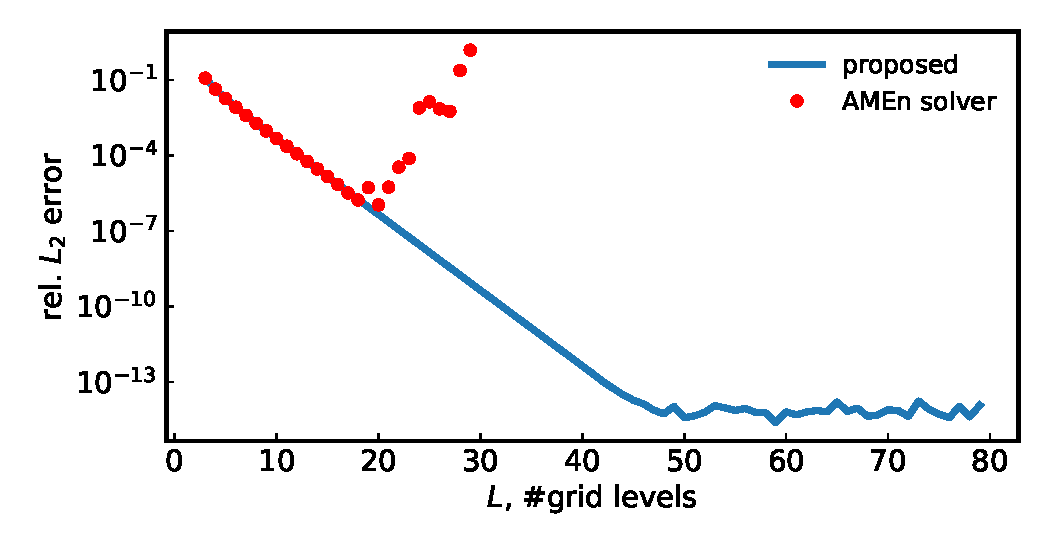
\includegraphics[width=0.65\textwidth]{robust.pdf}
	\caption{Относительные $\mathrm{L}_2$-ошибки относительно числа уровней сетки $\LL$ (общее число точек сетки равно $2^\LL$) для решений, полученных при решении $A_h u_h = f_h$ с помощью решателя AMEn и при прямом вычислении $u_h = A_h^{-1}f_h$ как QTT матрицы на векторное произведение по предложенным формулам для $A_h^{-1}$}.
	\label{fig:numerical}
\end{figure}

\begin{remark}
	Чтобы построить ядра QTT-разложения $A_h^{-1}$, нам нужно вычислить числа вида $z^M$ для $z = 1 - \gamma_1 h + \gamma_2 h^2 + O(h^3)$.
	Для больших значений $M$ (например, $M = 2^\LL$) и малых значений $h$ (например, $h \approx \sqrt{\varepsilon_{\mathrm{machine}}}$) прямое вычисление $z^M$ дает ошибку порядка $\sqrt{\varepsilon_{\mathrm{machine}}}$.
	Это происходит потому, что термин $\gamma_2h^2$ ``потерян'' во время вычисления $z$, в то время как следующее показывает, что он имеет $\mathcal{O}(h)$ влияние на $z^{2^L}$:
	\begin{align*}
	z^{2^L} &= z^{\frac{1}{h}} = \exp\left(\frac{1}{h}\ln(1 - \gamma_1 h + \gamma_2 h^2 + O(h^3))\right) = \\ &= \exp\left(\frac{1}{h}(-\gamma_1 h + (\gamma_2^2-\gamma_1^2)h^2 + O(h^3))\right)
	= \exp(-\gamma_1 + (\gamma_2^2 - \gamma_1^2)h + O(h^2)).
	\end{align*}
	Чтобы сохранить точность порядка $\varepsilon_{\mathrm{machine}}$, мы использовали приведенное выше расширение вместо наивного вычисления ~$z^M$.
\end{remark}


\section{Доказательства раздела~\ref{sec:circ}} \label{app:circ}

\begin{lemma}\label{lm:sum-shift}
	Для любой функции $f(j):\{0,\dots,N-1\}\to \mathbb{C}$ и целых чисел $s,t$ справедливо следующее:
	\[
	\sum_{j=s}^{s+N-1} f(j \bmod N) = \sum_{j=t}^{t+N-1} f(j \bmod N).
	\]
\end{lemma}
\begin{proof}[Доказательство леммы~\ref{lm:sum-shift}].
	Для любого целого числа $s$ последовательность
	\[
	\Big(s \bmod N, \dots, (s+N-1) \bmod N\Big)
	\]
	очевидно, является перестановкой $(0,\dots, N-1)$, поэтому
	\[
	\sum_{j=s}^{s+N-1} f(j \bmod N) = \sum_{j=0}^{N-1} f(j) = \sum_{j=t}^{t+N-1} f(j \bmod N).
	\]
\end{proof}
\begin{proof}[Доказательство леммы~\ref{lm:equivalent}].
	Начнем с~\eqref{eq:inverse} и заменим индекс суммирования на $j' = j - \ell$:
	\[
	\sum_{j'=-\ell}^{N-1-\ell} A_{((k-\ell)- j') \bmod N, 0}~b_{j'\bmod N}
	=
	\delta_{k,\ell},\quad k,\ell \in \{0, \dots, N-1\}.
	\]
	Мы можем применить лемму ~\ref{lm:sum-shift} к левой части равенства, так как суммарное выражение действительно является функцией $j' \bmod N$.
	Таким образом, получаем:
	\[
	\sum_{j'=0}^{N-1} A_{((k-\ell)- j') \bmod N, 0}~b_{j'}
	=
	\delta_{k,\ell},\quad k,\ell \in \{0, \dots, N-1\}.
	\]
	Левая часть равенства зависит только от $(k-\ell) \bmod N$, поэтому вместо уравнений $N^2$ можно эквивалентно записать только $N$:
	\[
	\sum_{j=0}^{N-1} A_{(k-j) \bmod N, 0}~b_j
	=
	\delta_{k,0},~ 0\le k \le N-1,\quad k,\ell \in \{0, \dots, N-1\}.
	\]
	Если подставить индекс суммирования в $j'' = k-j$ и учесть, что $x_j = \xi_{j}$ для $0\le j \le N-1$, то получим
	\[
	\sum_{j''=k-m-n+1}^{k} A_{j'' \bmod N, 0}~\xi_{k-j''} = \delta_{k,0}.
	\]
	Снова применим лемму ~\ref{lm:sum-shift} (бифинитный вектор $\xi$ является $N$-периодическим и, таким образом, зависит только от $j'' \bmod N$):
	\[
	\sum_{j''=-n}^{m-1}A_{j'' \bmod N, 0}~\xi_{k-j''} = \delta_{k,0}.
	\]
	Очевидно, что для $-n \le j'' \le m-1$ справедливо, что $A_{j'' \bmod N,0} = \Ainf_{j'', 0}$.
	Более того, $\Ainf_{j'', 0} = 0$ для $j'' \not\in [-n,m-1]$, поэтому получаем
	\[
	\sum_{j''=-\infty}^{\infty}\Ainf_{j'',0}~\xi_{k-j''} = \delta_{k,0}.
	\]
	Измените индекс суммирования обратно на $j = k-j''$:
	\[
	\sum_{j=-\infty}^{\infty}\Ainf_{k-j,0}~\xi_{j}
	=
	\sum_{j=-\infty}^{\infty}\Ainf_{k,j}~\xi_{j}
	=
	\delta_{k,0},
	,~ 0\le k \le N-1.
	\]
	Теперь возьмем любое $k' \in \mathbb{Z}$ и представим его как $k' = k + Nq$, где $q$ и $k$ - целые числа, такие, что $0 \le k \le N-1$.
	Изменив индекс суммирования на $j' = j - Nq$, мы можем записать:
	\[
	\sum_{j=-\infty}^{\infty}\Ainf_{k',j}\xi_{j}
	=
	\sum_{j'=-\infty}^{\infty}\Ainf_{k',j'+Nq}\xi_{j'}
	=
	\sum_{j'=-\infty}^{\infty}\Ainf_{k,j'}\xi_{j'}
	=
	\delta_{k,0}.
	\]
	Поэтому система уравнений~\eqref{eq:inverse} эквивалентна бесконечной системе уравнений
	\[
	\sum_{j=-\infty}^{\infty}\Ainf_{k,j}\xi_{j} = \delta_{k\bmod N,0},~k\in\mathbb{Z},
	\]
	что то же самое, что и $\Ainf\xi = \beta$.
\end{proof}

\begin{proof}[Доказательство леммы~\ref{lm:unnamed}].
	Вычислим элемент матрицы $\Ainf \Binf$:
	\begin{align*}
	\sum_{j=-\infty}^{\infty}\Ainf_{k, j}\Binf_{j, \ell}
	&=
	\sum_{j=-\infty}^{\infty}\Ainf_{k-j, 0}\Binf_{j, \ell}
	=
	\sum_{j'=-n}^{m-1}a_{j'}\Binf_{k-j', \ell}
	=\\&=
	\frac{1}{2\pi i}\oint_U\frac{1}{g(z)}\sum_{j'=-n}^{m-1}a_{j'}z^{l-k+j'-1}dz
	=
	\frac{1}{2\pi i}\oint_U\frac{g(z)}{g(z)}z^{l-k-1}dz.
	\end{align*}
	Но для любого целого числа $q$ это верно:
	\[
	\oint_U z^{q}dz
	=
	\begin{cases}
	2\pi i,&\text{if } q = -1,\\
	0,&\text{otherwise}.
	\end{cases}
	\]
	Таким образом, мы получаем
	\[
	\sum_{j=-\infty}^{\infty}\Ainf_{k, j}\Binf_{j, \ell} = \delta_{k,\ell} ~\Longleftrightarrow~\Ainf \Binf = I^{(\infty)}.
	\]
\end{proof}
\section{Доказательства раздела~\ref{sec:qtt_repr}} \label{app:qtt_repr}

\begin{proof}[Доказательство предложения~\ref{prop:sum_z}].
	Сначала мы представляем циркулянт с помощью перестановочной матрицы $\perm$:
	\[
	\invA_\LL = \sum_{i_1,\dots,i_\LL=0}^{1,\dots,1} \sum_{t=1}^r \alpha_t z_t^{\left(2^{\LL-1}i_{\LL} + \dots + 2^1 i_2 + i_1\right)} \perm_\LL^{\,\overline{i_1\dots, i_\LL}}.
	\]
	Затем воспользуемся результатом леммы ~\ref{lm:perm} для $\perm_\LL^{\,\overline{i_1\dots, i_\LL}}$ и полилинейностью разложения TT:
	\[
	\begin{split}
	\invA_\LL 
	&= \sum_{i_1,\dots,i_\LL=0}^{1,\dots,1}\ \sum_{t=1}^r
	\alpha_t
	z_t^{\left(2^{\LL-1}i_{\LL} + \dots + 2^1 i_2 + i_1\right)} \ U_{i_\LL} \Join V_{i_{\LL-1}} \Join \dots \Join V_{i_{2}} \Join W_{i_1}  
	= \\
	&=
	\sum_{t=1}^r \left( \sum_{i_\LL=0}^1 z_t^{2^{\LL-1}i_{\LL}} U_{i_\LL}  \right)
	\Join 
	\dots
	\Join 
	\left( \alpha_t \sum_{i_1=0}^1 z_t^{i_{1}} W_{i_1} \right) = \\
	&=
	\sum_{t=1}^r \left(U_0 + z_t^{2^{\LL-1}} U_1 \right) \Join \left(V_0 + z_t^{2^{\LL-2}} V_1 \right) \Join \dots \Join \left(V_0 + z_t^{2^{1}} V_1 \right) \Join \left(\alpha_t \left(W_0 + z_t W_1 \right) \right) \\
	&=
	{\widetilde Q}_1 \Join {\widetilde Q}_2 \Join \dots \Join {\widetilde Q}_d,
	\end{split}
	\]
	где благодаря лемме ~\ref{lm:sumtt} ядра ${\widetilde Q}_k$ являются блочными матрицами размера блока $2r \times 2r$ для $k=2,\dots,\LL-1$, $1\times 2r$ для $k=1$ и $2r\times 1$ для $k=\LL$, то есть это явное QTT-представление со всеми рангами, равными $2r$.
	На следующих этапах наша цель - найти линейные зависимости и уменьшить значения рангов до $(2, r+1, \dots, r+1)$.
	Для простоты изложения мы приводим доказательство для $r=2$. Обобщение на $r>2$ является простым.
	У нас есть
	\[
	\begin{split}
	{\widetilde Q}_1
	&= 
	\begin{bmatrix}
	I + q_{1,1} H & H + q_{1,1} I & I + q_{2,1} H & H + q_{2,1} I
	\end{bmatrix}
	\\
	&= 
	\begin{bmatrix}
	I & H
	\end{bmatrix}
	\Join
	\begin{bmatrix}
	1 & q_{1,1} & 1 & q_{2,1} \\
	q_{1,1} & 1 & q_{2,1} & 1
	\end{bmatrix}
	\end{split}
	\]
	Далее, обозначая $Q_1 = \begin{bmatrix} I & H \end{bmatrix}$, мы имеем
	\[
	{\widetilde Q}_1 \Join {\widetilde Q}_2 = \left(Q_1 \Join  
	\begin{bmatrix}
	1 & q_{1,1} & 1 & q_{2,1} \\
	q_{1,1} & 1 & q_{2,1} & 1
	\end{bmatrix}  \right)
	\Join
	{\widetilde Q}_2
	=
	Q_1 \Join  
	\left(
	\begin{bmatrix}
	1 & q_{1,1} & 1 & q_{2,1} \\
	q_{1,1} & 1 & q_{2,1} & 1
	\end{bmatrix}
	\Join
	{\widetilde Q}_2
	\right),
	\]
	где
	\begin{equation}\label{eq:proof:Q}
	{\widetilde Q}_k = 
	\begin{bmatrix}
	I + q_{1,k} J' & J' \\
	q_{1,k} J & J + q_{1,k} I \\
	& & I + q_{2,k} J' & J' \\
	& & q_{2,k} J & J + q_{2,k} I
	\end{bmatrix}, 
	\quad  
	k = 2,\dots,L-1.
	\end{equation}
	Используя тот факт, что $q_{t,1} = q_{t,2}^2$ для всех $t$, получаем:
	\[
	\begin{split}
	&\begin{bmatrix}
	1 & q_{1,1} & 1 & q_{2,1} \\
	q_{1,1} & 1 & q_{2,1} & 1
	\end{bmatrix}
	\Join
	{\widetilde Q}_2
	\\
	&=\begin{bmatrix}
	I + q_{1,2} J' + q_{1,2}^3 J & J' + q_{1,2}^2J + q_{1,2}^3 I & I + q_{2,2} J' + q_{2,2}^3 J & J' + q_{2,2}^2J + q_{2,2}^3 I \\
	q_{1,2}^2 I + q_{1,2}^3 J' + q_{1,2} J & q_{1,2}^2J'+ J + q_{1,2} I & q_{2,2}^2 I + q_{2,2}^3 J' + q_{2,2} J & q_{2,2}^2J'+ J + q_{2,2} I
	\end{bmatrix} 
	\\
	&= 
	\begin{bmatrix}
	I & J' + q_{1,2}^2 J &  J' + q_{2,2}^2 J \\
	O & q_{1,2}I + q_{1,2}^2 J' + J & q_{2,2}I + q_{2,2}^2 J' + J
	\end{bmatrix}
	\Join 
	\begin{bmatrix}
	1 & q_{1,2}^3 & 1 & q_{2,2}^3\\
	q_{1,2}& 1 & 0 & 0 \\
	0 & 0 & q_{2,2} & 1 
	\end{bmatrix}.
	\end{split} 
	\]
	В последнем уравнении мы получили факторизацию в произведение блочной матрицы $2\times 3$, которую обозначим как $Q_2$, на матрицу $3\times 4$, которую далее размножим до ${\widetilde Q}_3$ (см. \eqref{eq:proof:Q} для ${\widetilde Q}_3$):
	\[
	\begin{split}
	&\begin{bmatrix}
	1 & q_{1,2}^3 & 1 & q_{2,2}^3 \\
	q_{1,2}& 1 & 0 & 0 \\
	0 & 0 & q_{2,2} & 1 
	\end{bmatrix}
	\Join
	{\widetilde Q}_3 
	=
	\begin{bmatrix}
	1 & q_{1,3}^6 & 1 & q_{2,3}^6\\
	q_{1,3}^2& 1 & 0 & 0 \\
	0 & 0 & q_{2,3}^2 & 1 
	\end{bmatrix}
	\Join
	\begin{bmatrix}
	I + q_{1,3} J' & J' \\
	q_{1,3} J & J + q_{1,3} I \\
	& & I + q_{2,3} J' & J' \\
	& & q_{2,3} J & J + q_{2,3} I
	\end{bmatrix}
	\\
	& = 
	\begin{bmatrix}
	I + q_{1,3} J' + q_{1,3}^7 J & J' + q_{1,3}^6 J + q_{1,3}^7 I & I + q_{2,3} J' + q_{2,3}^7 J & J' + q_{2,3}^6 J + q_{2,3}^7 I \\
	q_{1,3}^2 I + q_{1,3}^3 J' + q_{1,3} J  & q_{1,3}^2 J' + J + q_{1,3} I & & \\
	& & q_{2,3}^2 I + q_{2,3}^3 J' + q_{2,3} J  & q_{2,3}^2 J' + J + q_{2,3} I 
	\end{bmatrix}
	\\
	& = 
	\begin{bmatrix}
	I & J' + q_{1,3}^6 J & J' + q_{2,3}^6 J \\
	& q_{1,3} I + q_{1,3}^2 J' + J \\
	& & q_{2,3} I + q_{2,3}^2 J' + J
	\end{bmatrix}
	\Join
	\begin{bmatrix}
	1 & q_{1,3}^7 & 1 & q_{2,3}^7 \\
	q_{1,3} & 1 & 0 & 0 \\
	0 & 0 & q_{2,3} & 1
	\end{bmatrix}
	\equiv 
	Q_3 \Join
	\begin{bmatrix}
	1 & q_{1,3}^7 & 1 & q_{2,3}^7 \\
	q_{1,3} & 1 & 0 & 0 \\
	0 & 0 & q_{2,3} & 1
	\end{bmatrix}.
	\end{split} 
	\]
	Распространяя его дальше, мы получаем следующее повторение:
	\[
	\begin{bmatrix}
	1 & q_{1,k-1}^{2^{k-1}-1} & 1 & q_{2,k-1}^{2^{k-1}-1} \\
	q_{1,k-1}& 1 & 0 & 0 \\
	0 & 0 & q_{2,k-1} & 1 
	\end{bmatrix}
	\Join
	{\widetilde Q}_k
	=
	Q_k \Join 
	\begin{bmatrix}
	1 & q_{1,k}^{2^{k}-1} & 1 & q_{2,k}^{2^{k}-1} \\
	q_{1,k}& 1 & 0 & 0 \\
	0 & 0 & q_{2,k} & 1 
	\end{bmatrix},
	\]
	где
	\[
	Q_k = 
	\begin{bmatrix}
	I & J' + q_{1,k}^{2^{k}-2} J & J' + q_{2,k}^{2^{k}-2} J \\
	& q_{1,k} I + q_{1,k}^2 J' + J \\
	& & q_{2,k} I + q_{2,k}^2 J' + J
	\end{bmatrix}.
	\]
	Для последнего ядра получаем:
	\[
	\begin{split}
	Q_\LL &=
	\begin{bmatrix}
	1 & q_{1,\LL-1}^{2^{\LL-1}-1} & 1 & q_{2,\LL-1}^{2^{\LL-1}-1} \\
	q_{1,\LL-1}& 1 & 0 & 0 \\
	0 & 0 & q_{2,\LL-1} & 1 
	\end{bmatrix}
	\Join
	{\widetilde Q}_\LL
	= 
	\begin{bmatrix}
	1 & q_{1,\LL}^{2^{\LL}-2} & 1 & q_{2,\LL}^{2^{\LL}-2} \\
	q_{1,\LL}^2 & 1 & 0 & 0 \\
	0 & 0 & q_{2,\LL}^2 & 1
	\end{bmatrix}
	\Join
	\begin{bmatrix}
	\alpha_1 \left(I + q_{1,\LL}J' \right) \\
	\alpha_1 q_{1,\LL} J \\
	\alpha_2 \left(I + q_{2,\LL}J' \right) \\
	\alpha_2 q_{2,\LL} J 
	\end{bmatrix}
	\\
	&= 
	\begin{bmatrix}
	(\alpha_1 + \alpha_2) I + (\alpha_1 q_{1,\LL} + \alpha_2 q_{2,\LL}) J' + (\alpha_1 q_{1,\LL}^{2^{\LL}-1}+ \alpha_2 q_{1,\LL}^{2^{\LL}-1}) J \\
	\alpha_1 q_{1,\LL} \left(J + q_{2,\LL}I + q_{1,\LL}^2 J' \right)\\
	\alpha_2 q_{2,\LL} \left(J + q_{2,\LL}I + q_{2,\LL}^2 J' \right)
	\end{bmatrix}
	\end{split}
	\]
\end{proof}



\section{Доказательства раздела~\ref{sec:examples}} \label{app:examples}


\begin{proof}[Доказательство предложения~\ref{prop:laur_prod}].
	Вычислим первый столбец циркулянта $C = AB$.
	\begin{align*}
	C_{s,0}
	&=
	\sum_{t=0}^{N-1} A_{s,t}B_{t,0}
	=
	\sum_{t=0}^{N-1} A_{s-t \bmod N,0}~B_{t,0}
	= \\ &=
	\sum_{t=0}^{m_B-1} A_{s-t \bmod N,0}~B_{t,0}
	+
	\sum_{t=-n_B}^{-1} A_{s-(N+t) \bmod N,0}~B_{N+t,0}.
	\end{align*}
	Если обозначить $a_t$ и $b_t$ коэффициентами полиномов Лорана $f_A(z)$ и $f_B(z)$ соответственно, то можно упростить приведенное выше выражение:
	\[
	C_{s, 0} = \sum_{t=-n_B}^{m_B-1} A_{s-t \bmod N,0}~b_t.
	\]
	Теперь мы разбиваем набор индексов строк $s$ на три части:
	\begin{align*}
	S_1 &= \{0, \dots, m_A+m_B-2\},\\
	S_2 &= \{m_A+m_B-1, \dots, N-n_A-n_B-1\}, \\
	S_3 &=\{N-n_A-n_B,\dots,N-1\}.    
	\end{align*}
	%	
	Если $s \in S_1$, то $(s-t) \in [-m_A, m_A+m_B-2+n_B]$, и мы можем написать $A_{s-t \bmod N, 0} = a_{s-t}$ (здесь мы подразумеваем, что $a_i = 0$ для $i \not\in [-n_A, m_B-1]$).
	Далее, если $s \in S_2$, то $(s-t) \in [m_A, N-n_A-1]$, следовательно, $A_{s-t \bmod N,0} = 0$.
	Наконец, если $s \in S_3$, то $(s-t) \in [N-n_A-n_B-m_B+1, N-1+n_B]$ и $A_{s-t \bmod N, 0} = a_{s-t-N}$.
	Если взять три случая вместе и использовать обозначения $m = m_A + m_B$, $n=n_A + n_B$, то можно написать
	\begin{equation}\label{eq:C-s}
	C_{s,0} = \begin{cases}
	\sum_{t=-n_B}^{m_B-1} a_{s-t}b_t,
	&\text{ if } s \in [0, m-1],\\
	0, &\text{ if } s \in [m, N-n-1], \\
	\sum_{t=-n_B}^{m_B-1} a_{s-t-N}b_t, & \text{ if } s \in [N-n, N-1].
	\end{cases}
	\end{equation}
	Итак, циркулянт $C$ действительно имеет вид~\eqref{eq:A} с параметрами $m$ и $n$ (свойства $c_{m-1} \neq 0$ и $c_{-n} \neq 0$ будут проверены чуть позже).
	Более того, как и для $s \in [-n,-1]$ мы имеем по определению
	$c_s = C_{N+s, 0}$, из~\eqref{eq:C-s} следует, что общая формула для $c_s$ имеет вид
	\[
	c_s = \sum_{t=-n_B}^{m_B-1} a_{s-t}b_t~~\text{ for all } s \in \{-n, \dots, m-1\}.
	\]
	Это в точности формула произведения полиномов Лорана $f_A(z)$ и $f_B(z)$.
	Наконец, нам нужно доказать, что $c_{m-1}$ и $c_{-n}$ ненулевые.
	По~\eqref{eq:C-s}, $c_{m-1} = a_{m_A-1}b_{m_B-1} \neq 0$ как $a_{m_A-1}$ и $b_{m_B-1}$ ненулевые.
	Аналогично, $c_{-n} = a_{-n_A}b_{-n_B} \neq 0$.
\end{proof}



\section{Форматирование текста}\label{sec:ch1/sec1}

Мы можем сделать \textbf{жирный текст} и \textit{курсив}.

\section{Ссылки}\label{sec:ch1/sec2}

Сошлёмся на библиографию.
Одна ссылка: \cite[с.~54]{Sokolov}\cite[с.~36]{Gaidaenko}.
Две ссылки: \cite{Sokolov,Gaidaenko}.
Ссылка на собственные работы: \cite{vakbib1, confbib2}.
Много ссылок: %\cite[с.~54]{Lermontov,Management,Borozda} % такой «фокус»
%вызывает biblatex warning относительно опции sortcites, потому что неясно, к
%какому источнику относится уточнение о страницах, а bibtex об этой проблеме
%даже не предупреждает
\cite{Lermontov, Management, Borozda, Marketing, Constitution, FamilyCode,
    Gost.7.0.53, Razumovski, Lagkueva, Pokrovski, Methodology, Berestova,
    Kriger}%
\ifnumequal{\value{bibliosel}}{0}{% Примеры для bibtex8
    \cite{Sirotko, Lukina, Encyclopedia, Nasirova}%
}{% Примеры для biblatex через движок biber
    \cite{Sirotko2, Lukina2, Encyclopedia2, Nasirova2}%
}%
.
И~ещё немного ссылок:~\cite{Article,Book,Booklet,Conference,Inbook,Incollection,Manual,Mastersthesis,
    Misc,Phdthesis,Proceedings,Techreport,Unpublished}
% Следует обратить внимание, что пробел после запятой внутри \cite{}
% обрабатывается ожидаемо, а пробел перед запятой, может вызывать проблемы при
% обработке ссылок.
\cite{medvedev2006jelektronnye, CEAT:CEAT581, doi:10.1080/01932691.2010.513279,
    Gosele1999161,Li2007StressAnalysis, Shoji199895, test:eisner-sample,
    test:eisner-sample-shorted, AB_patent_Pomerantz_1968, iofis_patent1960}%
\ifnumequal{\value{bibliosel}}{0}{% Примеры для bibtex8
}{% Примеры для biblatex через движок biber
    \cite{patent2h, patent3h, patent2}%
}%
.

\ifnumequal{\value{bibliosel}}{0}{% Примеры для bibtex8
Попытка реализовать несколько ссылок на конкретные страницы
для \texttt{bibtex} реализации библиографии:
[\citenum{Sokolov}, с.~54; \citenum{Gaidaenko}, с.~36].
}{% Примеры для biblatex через движок biber
Несколько источников (мультицитата):
% Тут специально написано по-разному тире, для демонстрации, что
% применение специальных тире в настоящий момент в biblatex приводит к непоказу
% "с.".
\cites[vii--x, 5, 7]{Sokolov}[v"--~x, 25, 526]{Gaidaenko}[vii--x, 5, 7]{Techreport},
работает только в \texttt{biblatex} реализации библиографии.
}%

Ссылки на собственные работы:~\cite{vakbib1, confbib1}.

Сошлёмся на приложения: Приложение~\cref{app:A}, Приложение~\cref{app:B2}.

Сошлёмся на формулу: формула~\cref{eq:equation1}.

Сошлёмся на изображение: рисунок~\cref{fig:knuth}.

Стандартной практикой является добавление к ссылкам префикса, характеризующего тип элемента.
Это не является строгим требованием, но~позволяет лучше ориентироваться в документах большого размера.
Например, для ссылок на~рисунки используется префикс \textit{fig},
для ссылки на~таблицу "--- \textit{tab}.

В таблице \cref{tab:tab_pref} приложения~\cref{app:B4} приведён список рекомендуемых
к использованию стандартных префиксов.

В некоторых ситуациях возникает необходимость отойти от требований ГОСТ по оформлению ссылок на
литературу.
В таком случае можно воспользоваться дополнительными опциями пакета \verb+biblatex+.

Например, в ссылке на книгу~\cite{sobenin_kdv} использование опции \verb+maxnames=4+ позволяет
вывести имена всех четырёх авторов.
По ГОСТ имена последних трёх авторов опускаются.

Кроме того, часто возникают проблемы с транслитерованными инициалами. Некоторые буквы русского
алфавита по правилам транслитерации записываются двумя буквами латинского алфавита (ю-yu, ё-yo и
т.д.).
Такие инициалы \verb+biblatex+ будет сокращать до одной буквы, что неверно.
Поправить его работу можно использовав опцию \verb+giveninits=false+.
Пример использования этой опции можно видеть в ссылке~\cite{initials}.

\section{Формулы}\label{sec:ch1/sec3}

Благодаря пакету \textit{icomma}, \LaTeX~одинаково хорошо воспринимает
в~качестве десятичного разделителя и запятую (\(3,1415\)), и точку (\(3.1415\)).

\subsection{Ненумерованные одиночные формулы}\label{subsec:ch1/sec3/sub1}

Вот так может выглядеть формула, которую необходимо вставить в~строку
по~тексту: \(x \approx \sin x\) при \(x \to 0\).

А вот так выглядит ненумерованная отдельностоящая формула c подстрочными
и надстрочными индексами:
\[
    (x_1+x_2)^2 = x_1^2 + 2 x_1 x_2 + x_2^2
\]

Формула с неопределенным интегралом:
\[
    \int f(\alpha+x)=\sum\beta
\]

При использовании дробей формулы могут получаться очень высокие:
\[
    \frac{1}{\sqrt{2}+
        \displaystyle\frac{1}{\sqrt{2}+
            \displaystyle\frac{1}{\sqrt{2}+\cdots}}}
\]

В формулах можно использовать греческие буквы:
%Все \original... команды заранее, ради этого примера, определены в Dissertation\userstyles.tex
\[
    \alpha\beta\gamma\delta\originalepsilon\epsilon\zeta\eta\theta%
    \vartheta\iota\kappa\varkappa\lambda\mu\nu\xi\pi\varpi\rho\varrho%
    \sigma\varsigma\tau\upsilon\originalphi\phi\chi\psi\omega\Gamma\Delta%
    \Theta\Lambda\Xi\Pi\Sigma\Upsilon\Phi\Psi\Omega
\]
\[%https://texfaq.org/FAQ-boldgreek
    \boldsymbol{\alpha\beta\gamma\delta\originalepsilon\epsilon\zeta\eta%
        \theta\vartheta\iota\kappa\varkappa\lambda\mu\nu\xi\pi\varpi\rho%
        \varrho\sigma\varsigma\tau\upsilon\originalphi\phi\chi\psi\omega\Gamma%
        \Delta\Theta\Lambda\Xi\Pi\Sigma\Upsilon\Phi\Psi\Omega}
\]

Для добавления формул можно использовать пары \verb+$+\dots\verb+$+ и \verb+$$+\dots\verb+$$+,
но~они считаются устаревшими.
Лучше использовать их функциональные аналоги \verb+\(+\dots\verb+\)+ и \verb+\[+\dots\verb+\]+.

\subsection{Ненумерованные многострочные формулы}\label{subsec:ch1/sec3/sub2}

Вот так можно написать две формулы, не нумеруя их, чтобы знаки <<равно>> были
строго друг под другом:
\begin{align}
    f_W & =  \min \left( 1, \max \left( 0, \frac{W_{soil} / W_{max}}{W_{crit}} \right)  \right), \nonumber \\
    f_T & =  \min \left( 1, \max \left( 0, \frac{T_s / T_{melt}}{T_{crit}} \right)  \right), \nonumber
\end{align}

Выровнять систему ещё и по переменной \( x \) можно, используя окружение
\verb|alignedat| из пакета \verb|amsmath|. Вот так:
\[
|x| = \left\{
\begin{alignedat}{2}
    &&x, \quad &\text{eсли } x\geqslant 0 \\
    &-&x, \quad & \text{eсли } x<0
\end{alignedat}
\right.
\]
Здесь первый амперсанд (в исходном \LaTeX\ описании формулы) означает
выравнивание по~левому краю, второй "--- по~\( x \), а~третий "--- по~слову
<<если>>. Команда \verb|\quad| делает большой горизонтальный пробел.

Ещё вариант:
\[
    |x|=
    \begin{cases}
        \phantom{-}x, \text{если } x \geqslant 0 \\
        -x, \text{если } x<0
    \end{cases}
\]

Кроме того, для  нумерованных формул \verb|alignedat| делает вертикальное
выравнивание номера формулы по центру формулы. Например, выравнивание
компонент вектора:
\begin{equation}
    \label{eq:2p3}
    \begin{alignedat}{2}
        {\mathbf{N}}_{o1n}^{(j)} = \,{\sin} \phi\,n\!\left(n+1\right)
        {\sin}\theta\,
        \pi_n\!\left({\cos} \theta\right)
        \frac{
        z_n^{(j)}\!\left( \rho \right)
        }{\rho}\,
        &{\boldsymbol{\hat{\mathrm e}}}_{r}\,+   \\
        +\,
        {\sin} \phi\,
        \tau_n\!\left({\cos} \theta\right)
        \frac{
        \left[\rho z_n^{(j)}\!\left( \rho \right)\right]^{\prime}
        }{\rho}\,
        &{\boldsymbol{\hat{\mathrm e}}}_{\theta}\,+   \\
        +\,
        {\cos} \phi\,
        \pi_n\!\left({\cos} \theta\right)
        \frac{
        \left[\rho z_n^{(j)}\!\left( \rho \right)\right]^{\prime}
        }{\rho}\,
        &{\boldsymbol{\hat{\mathrm e}}}_{\phi}\:.
    \end{alignedat}
\end{equation}

Ещё об отступах. Иногда для лучшей <<читаемости>> формул полезно
немного исправить стандартные интервалы \LaTeX\ с учётом логической
структуры самой формулы. Например в формуле~\cref{eq:2p3} добавлен
небольшой отступ \verb+\,+ между основными сомножителями, ниже
результат применения всех вариантов отступа:
\begin{align*}
    \backslash!             & \quad f(x) = x^2\! +3x\! +2         \\
    \mbox{по-умолчанию}     & \quad f(x) = x^2+3x+2               \\
    \backslash,             & \quad f(x) = x^2\, +3x\, +2         \\
    \backslash{:}           & \quad f(x) = x^2\: +3x\: +2         \\
    \backslash;             & \quad f(x) = x^2\; +3x\; +2         \\
    \backslash \mbox{space} & \quad f(x) = x^2\ +3x\ +2           \\
    \backslash \mbox{quad}  & \quad f(x) = x^2\quad +3x\quad +2   \\
    \backslash \mbox{qquad} & \quad f(x) = x^2\qquad +3x\qquad +2
\end{align*}

Можно использовать разные математические алфавиты:
\begin{align}
    \mathcal{ABCDEFGHIJKLMNOPQRSTUVWXYZ} \nonumber  \\
    \mathfrak{ABCDEFGHIJKLMNOPQRSTUVWXYZ} \nonumber \\
    \mathbb{ABCDEFGHIJKLMNOPQRSTUVWXYZ} \nonumber
\end{align}

Посмотрим на систему уравнений на примере аттрактора Лоренца:

\[
\left\{
\begin{array}{rl}
    \dot x = & \sigma (y-x)  \\
    \dot y = & x (r - z) - y \\
    \dot z = & xy - bz
\end{array}
\right.
\]

А для вёрстки матриц удобно использовать многоточия:
\[
    \left(
        \begin{array}{ccc}
            a_{11} & \ldots & a_{1n} \\
            \vdots & \ddots & \vdots \\
            a_{n1} & \ldots & a_{nn} \\
        \end{array}
    \right)
\]

\subsection{Нумерованные формулы}\label{subsec:ch1/sec3/sub3}

А вот так пишется нумерованная формула:
\begin{equation}
    \label{eq:equation1}
    e = \lim_{n \to \infty} \left( 1+\frac{1}{n} \right) ^n
\end{equation}

Нумерованных формул может быть несколько:
\begin{equation}
    \label{eq:equation2}
    \lim_{n \to \infty} \sum_{k=1}^n \frac{1}{k^2} = \frac{\pi^2}{6}
\end{equation}

Впоследствии на формулы~\cref{eq:equation1, eq:equation2} можно ссылаться.

Сделать так, чтобы номер формулы стоял напротив средней строки, можно,
используя окружение \verb|multlined| (пакет \verb|mathtools|) вместо
\verb|multline| внутри окружения \verb|equation|. Вот так:
\begin{equation} % \tag{S} % tag - вписывает свой текст
    \label{eq:equation3}
    \begin{multlined}
        1+ 2+3+4+5+6+7+\dots + \\
        + 50+51+52+53+54+55+56+57 + \dots + \\
        + 96+97+98+99+100=5050
    \end{multlined}
\end{equation}

Уравнения~\cref{eq:subeq_1,eq:subeq_2} демонстрируют возможности
окружения \verb|\subequations|.
\begin{subequations}
    \label{eq:subeq_1}
    \begin{gather}
        y = x^2 + 1 \label{eq:subeq_1-1} \\
        y = 2 x^2 - x + 1 \label{eq:subeq_1-2}
    \end{gather}
\end{subequations}
Ссылки на отдельные уравнения~\cref{eq:subeq_1-1,eq:subeq_1-2,eq:subeq_2-1}.
\begin{subequations}
    \label{eq:subeq_2}
    \begin{align}
        y & = x^3 + x^2 + x + 1 \label{eq:subeq_2-1} \\
        y & = x^2
    \end{align}
\end{subequations}

\subsection{Форматирование чисел и размерностей величин}\label{sec:units}

Числа форматируются при помощи команды \verb|\num|:
\num{5,3};
\num{2,3e8};
\num{12345,67890};
\num{2,6 d4};
\num{1+-2i};
\num{.3e45};
\num[exponent-base=2]{5 e64};
\num[exponent-base=2,exponent-to-prefix]{5 e64};
\num{1.654 x 2.34 x 3.430}
\num{1 2 x 3 / 4}.
Для написания последовательности чисел можно использовать команды \verb|\numlist| и \verb|\numrange|:
\numlist{10;30;50;70}; \numrange{10}{30}.
Значения углов можно форматировать при помощи команды \verb|\ang|:
\ang{2.67};
\ang{30,3};
\ang{-1;;};
\ang{;-2;};
\ang{;;-3};
\ang{300;10;1}.

Обратите внимание, что ГОСТ запрещает использование знака <<->> для обозначения отрицательных чисел
за исключением формул, таблиц и~рисунков.
Вместо него следует использовать слово <<минус>>.

Размерности можно записывать при помощи команд \verb|\si| и \verb|\SI|:
\si{\farad\squared\lumen\candela};
\si{\joule\per\mole\per\kelvin};
\si[per-mode = symbol-or-fraction]{\joule\per\mole\per\kelvin};
\si{\metre\per\second\squared};
\SI{0.10(5)}{\neper};
\SI{1.2-3i e5}{\joule\per\mole\per\kelvin};
\SIlist{1;2;3;4}{\tesla};
\SIrange{50}{100}{\volt}.
Список единиц измерений приведён в таблицах~\cref{tab:unit:base,
    tab:unit:derived,tab:unit:accepted,tab:unit:physical,tab:unit:other}.
Приставки единиц приведены в~таблице~\cref{tab:unit:prefix}.

С дополнительными опциями форматирования можно ознакомиться в~описании пакета \texttt{siunitx};
изменить или добавить единицы измерений можно в~файле \texttt{siunitx.cfg}.

\begin{table}
    \centering
    \captionsetup{justification=centering} % выравнивание подписи по-центру
    \caption{Основные величины СИ}\label{tab:unit:base}
    \begin{tabular}{llc}
        \toprule
        Название  & Команда                 & Символ         \\
        \midrule
        Ампер     & \verb|\ampere| & \si{\ampere}   \\
        Кандела   & \verb|\candela| & \si{\candela}  \\
        Кельвин   & \verb|\kelvin| & \si{\kelvin}   \\
        Килограмм & \verb|\kilogram| & \si{\kilogram} \\
        Метр      & \verb|\metre| & \si{\metre}    \\
        Моль      & \verb|\mole| & \si{\mole}     \\
        Секунда   & \verb|\second| & \si{\second}   \\
        \bottomrule
    \end{tabular}
\end{table}

\begin{table}
    \small
    \centering
    \begin{threeparttable}% выравнивание подписи по границам таблицы
        \caption{Производные единицы СИ}\label{tab:unit:derived}
        \begin{tabular}{llc|llc}
            \toprule
            Название       & Команда                 & Символ              & Название & Команда & Символ \\
            \midrule
            Беккерель      & \verb|\becquerel| & \si{\becquerel}     &
            Ньютон         & \verb|\newton| & \si{\newton}                                      \\
            Градус Цельсия & \verb|\degreeCelsius| & \si{\degreeCelsius} &
            Ом             & \verb|\ohm| & \si{\ohm}                                         \\
            Кулон          & \verb|\coulomb| & \si{\coulomb}       &
            Паскаль        & \verb|\pascal| & \si{\pascal}                                      \\
            Фарад          & \verb|\farad| & \si{\farad}         &
            Радиан         & \verb|\radian| & \si{\radian}                                      \\
            Грей           & \verb|\gray| & \si{\gray}          &
            Сименс         & \verb|\siemens| & \si{\siemens}                                     \\
            Герц           & \verb|\hertz| & \si{\hertz}         &
            Зиверт         & \verb|\sievert| & \si{\sievert}                                     \\
            Генри          & \verb|\henry| & \si{\henry}         &
            Стерадиан      & \verb|\steradian| & \si{\steradian}                                   \\
            Джоуль         & \verb|\joule| & \si{\joule}         &
            Тесла          & \verb|\tesla| & \si{\tesla}                                       \\
            Катал          & \verb|\katal| & \si{\katal}         &
            Вольт          & \verb|\volt| & \si{\volt}                                        \\
            Люмен          & \verb|\lumen| & \si{\lumen}         &
            Ватт           & \verb|\watt| & \si{\watt}                                        \\
            Люкс           & \verb|\lux| & \si{\lux}           &
            Вебер          & \verb|\weber| & \si{\weber}                                       \\
            \bottomrule
        \end{tabular}
    \end{threeparttable}
\end{table}

\begin{table}
    \centering
    \begin{threeparttable}% выравнивание подписи по границам таблицы
        \caption{Внесистемные единицы}\label{tab:unit:accepted}

        \begin{tabular}{llc}
            \toprule
            Название        & Команда                 & Символ          \\
            \midrule
            День            & \verb|\day| & \si{\day}       \\
            Градус          & \verb|\degree| & \si{\degree}    \\
            Гектар          & \verb|\hectare| & \si{\hectare}   \\
            Час             & \verb|\hour| & \si{\hour}      \\
            Литр            & \verb|\litre| & \si{\litre}     \\
            Угловая минута  & \verb|\arcminute| & \si{\arcminute} \\
            Угловая секунда & \verb|\arcsecond| & \si{\arcsecond} \\ %
            Минута          & \verb|\minute| & \si{\minute}    \\
            Тонна           & \verb|\tonne| & \si{\tonne}     \\
            \bottomrule
        \end{tabular}
    \end{threeparttable}
\end{table}

\begin{table}
    \centering
    \captionsetup{justification=centering}
    \caption{Внесистемные единицы, получаемые из эксперимента}\label{tab:unit:physical}
    \begin{tabular}{llc}
        \toprule
        Название                & Команда                 & Символ                 \\
        \midrule
        Астрономическая единица & \verb|\astronomicalunit| & \si{\astronomicalunit} \\
        Атомная единица массы   & \verb|\atomicmassunit| & \si{\atomicmassunit}   \\
        Боровский радиус        & \verb|\bohr| & \si{\bohr}             \\
        Скорость света          & \verb|\clight| & \si{\clight}           \\
        Дальтон                 & \verb|\dalton| & \si{\dalton}           \\
        Масса электрона         & \verb|\electronmass| & \si{\electronmass}     \\
        Электрон Вольт          & \verb|\electronvolt| & \si{\electronvolt}     \\
        Элементарный заряд      & \verb|\elementarycharge| & \si{\elementarycharge} \\
        Энергия Хартри          & \verb|\hartree| & \si{\hartree}          \\
        Постоянная Планка       & \verb|\planckbar| & \si{\planckbar}        \\
        \bottomrule
    \end{tabular}
\end{table}

\begin{table}
    \centering
    \begin{threeparttable}% выравнивание подписи по границам таблицы
        \caption{Другие внесистемные единицы}\label{tab:unit:other}
        \begin{tabular}{llc}
            \toprule
            Название                  & Команда                 & Символ             \\
            \midrule
            Ангстрем                  & \verb|\angstrom| & \si{\angstrom}     \\
            Бар                       & \verb|\bar| & \si{\bar}          \\
            Барн                      & \verb|\barn| & \si{\barn}         \\
            Бел                       & \verb|\bel| & \si{\bel}          \\
            Децибел                   & \verb|\decibel| & \si{\decibel}      \\
            Узел                      & \verb|\knot| & \si{\knot}         \\
            Миллиметр ртутного столба & \verb|\mmHg| & \si{\mmHg}         \\
            Морская миля              & \verb|\nauticalmile| & \si{\nauticalmile} \\
            Непер                     & \verb|\neper| & \si{\neper}        \\
            \bottomrule
        \end{tabular}
    \end{threeparttable}
\end{table}

\begin{table}
    \small
    \centering
    \begin{threeparttable}% выравнивание подписи по границам таблицы
        \caption{Приставки СИ}\label{tab:unit:prefix}
        \begin{tabular}{llcc|llcc}
            \toprule
            Приставка & Команда                  & Символ      & Степень &
            Приставка & Команда                  & Символ      & Степень   \\
            \midrule
            Иокто     & \verb|\yocto|  & \si{\yocto} & -24     &
            Дека      & \verb|\deca|  & \si{\deca}  & 1         \\
            Зепто     & \verb|\zepto|  & \si{\zepto} & -21     &
            Гекто     & \verb|\hecto|  & \si{\hecto} & 2         \\
            Атто      & \verb|\atto|  & \si{\atto}  & -18     &
            Кило      & \verb|\kilo|  & \si{\kilo}  & 3         \\
            Фемто     & \verb|\femto|  & \si{\femto} & -15     &
            Мега      & \verb|\mega|  & \si{\mega}  & 6         \\
            Пико      & \verb|\pico|  & \si{\pico}  & -12     &
            Гига      & \verb|\giga|  & \si{\giga}  & 9         \\
            Нано      & \verb|\nano|  & \si{\nano}  & -9      &
            Терра     & \verb|\tera|  & \si{\tera}  & 12        \\
            Микро     & \verb|\micro|  & \si{\micro} & -6      &
            Пета      & \verb|\peta|  & \si{\peta}  & 15        \\
            Милли     & \verb|\milli|  & \si{\milli} & -3      &
            Екса      & \verb|\exa|  & \si{\exa}   & 18        \\
            Санти     & \verb|\centi|  & \si{\centi} & -2      &
            Зетта     & \verb|\zetta|  & \si{\zetta} & 21        \\
            Деци      & \verb|\deci| & \si{\deci}  & -1      &
            Иотта     & \verb|\yotta| & \si{\yotta} & 24        \\
            \bottomrule
        \end{tabular}
    \end{threeparttable}
\end{table}

\subsection{Заголовки с формулами: \texorpdfstring{\(a^2 + b^2 = c^2\)}{%
        a\texttwosuperior\ + b\texttwosuperior\ = c\texttwosuperior},
    \texorpdfstring{\(\left\vert\textrm{{Im}}\Sigma\left(
            \protect\varepsilon\right)\right\vert\approx const\)}{|ImΣ (ε)| ≈ const},
    \texorpdfstring{\(\sigma_{xx}^{(1)}\)}{σ\_\{xx\}\textasciicircum\{(1)\}}
}\label{subsec:with_math}

Пакет \texttt{hyperref} берёт текст для закладок в pdf-файле из~аргументов
команд типа \verb|\section|, которые могут содержать математические формулы,
а~также изменения цвета текста или шрифта, которые не отображаются в~закладках.
Чтобы использование формул в заголовках не вызывало в~логе компиляции появление
предупреждений типа <<\texttt{Token not allowed in~a~PDF string
    (Unicode):(hyperref) removing...}>>, следует использовать конструкцию
\verb|\texorpdfstring{}{}|, где в~первых фигурных скобках указывается
формула, а~во~вторых "--- запись формулы для закладок.

\section{Рецензирование текста}\label{sec:markup}

В шаблоне для диссертации и автореферата заданы команды рецензирования.
Они видны при компиляции шаблона в режиме черновика или при установке
соответствующей настройки (\verb+showmarkup+) в~файле \verb+common/setup.tex+.

Команда \verb+\todo+ отмечает текст красным цветом.
\todo{Например, так.}

Команда \verb+\note+ позволяет выбрать цвет текста.
\note{Чёрный, } \note[red]{красный, } \note[green]{зелёный, }
\note[blue]{синий.} \note[orange]{Обратите внимание на ширину и расстановку
    формирующихся пробелов, в~результате приведённой записи (зависит также
    от~применяемого компилятора).}

Окружение \verb+commentbox+ также позволяет выбрать цвет.

\begin{commentbox}[red]
    Красный текст.

    Несколько параграфов красного текста.
\end{commentbox}

\begin{commentbox}[blue]
    Синяя формула.

    \begin{equation}
        \alpha + \beta = \gamma
    \end{equation}
\end{commentbox}

\verb+commentbox+ позволяет закомментировать участок кода в~режиме чистовика.
Чтобы убрать кусок кода для всех режимов, можно использовать окружение
\verb+comment+.

\begin{comment}
Этот текст всегда скрыт.
\end{comment}

\section{Работа со списком сокращений и~условных обозначений}\label{sec:acronyms}

С помощью пакета \texttt{nomencl} можно создавать удобный сортированный список
сокращений и условных обозначений во время написания текста. Вызов
\verb+\nomenclature+ добавляет нужный символ или сокращение с~описанием
в~список, который затем печатается вызовом \verb+\printnomenclature+
в~соответствующем разделе.
Для того, чтобы эти операции прошли, потребуется дополнительный вызов
\verb+makeindex -s nomencl.ist -o %.nls %.nlo+ в~командной строке, где вместо
\verb+%+ следует подставить имя главного файла проекта (\verb+dissertation+
для этого шаблона).
Затем потребуется один или два дополнительных вызова компилятора проекта.
\begin{equation}
    \omega = c k,
\end{equation}
где \( \omega \) "--- частота света, \( c \) "--- скорость света, \( k \) "---
модуль волнового вектора.
\nomenclature{\(\omega\)}{частота света\nomrefeq}
\nomenclature{\(c\)}{скорость света\nomrefpage}
\nomenclature{\(k\)}{модуль волнового вектора\nomrefeqpage}
Использование
\begin{verbatim}
\nomenclature{\(\omega\)}{частота света\nomrefeq}
\nomenclature{\(c\)}{скорость света\nomrefpage}
\nomenclature{\(k\)}{модуль волнового вектора\nomrefeqpage}
\end{verbatim}
после уравнения добавит в список условных обозначений три записи.
Ссылки \verb+\nomrefeq+ на последнее уравнение, \verb+\nomrefpage+ "--- на
страницу, \verb+\nomrefeqpage+ "--- сразу на~последнее уравнение и~на~страницу,
можно опускать и~не~использовать.

Группировкой и сортировкой пунктов в списке можно управлять с~помощью указания
дополнительных аргументов к команде \verb+nomenclature+.
Например, при вызове
\begin{verbatim}
\nomenclature[03]{\( \hbar \)}{постоянная Планка}
\nomenclature[01]{\( G \)}{гравитационная постоянная}
\end{verbatim}
\( G \) будет стоять в списке выше, чем \( \hbar \).
Для корректных вертикальных отступов между строками в описании лучше
не~использовать многострочные формулы в~списке обозначений.

\nomenclature{%
    \( \begin{rcases}
        a_n \\
        b_n
    \end{rcases} \)%
}{коэффициенты разложения Ми в дальнем поле соответствующие электрическим и
    магнитным мультиполям}
\nomenclature[a\( e \)]{\( {\boldsymbol{\hat{\mathrm e}}} \)}{единичный вектор}
\nomenclature{\( E_0 \)}{амплитуда падающего поля}
\nomenclature{\( j \)}{тип функции Бесселя}
\nomenclature{\( k \)}{волновой вектор падающей волны}
\nomenclature{%
    \( \begin{rcases}
        a_n \\
        b_n
    \end{rcases} \)%
}{и снова коэффициенты разложения Ми в дальнем поле соответствующие
    электрическим и магнитным мультиполям. Добавлено много текста, так что
    описание группы условных обозначений значительно превысило высоту этой
    группы...}
\nomenclature{\( L \)}{общее число слоёв}
\nomenclature{\( l \)}{номер слоя внутри стратифицированной сферы}
\nomenclature{\( \lambda \)}{длина волны электромагнитного излучения в вакууме}
\nomenclature{\( n \)}{порядок мультиполя}
\nomenclature{%
    \( \begin{rcases}
        {\mathbf{N}}_{e1n}^{(j)} & {\mathbf{N}}_{o1n}^{(j)} \\
        {\mathbf{M}_{o1n}^{(j)}} & {\mathbf{M}_{e1n}^{(j)}}
    \end{rcases} \)%
}{сферические векторные гармоники}
\nomenclature{\( \mu \)}{магнитная проницаемость в вакууме}
\nomenclature{\( r, \theta, \phi \)}{полярные координаты}
\nomenclature{\( \omega \)}{частота падающей волны}

С помощью \verb+nomenclature+ можно включать в~список сокращения,
не~используя их~в~тексте.
% запись сокращения в список происходит командой \nomenclature,
% а не употреблением самого сокращения
\nomenclature{FEM}{finite element method, метод конечных элементов}
\nomenclature{FIT}{finite integration technique, метод конечных интегралов}
\nomenclature{FMM}{fast multipole method, быстрый метод многополюсника}
\nomenclature{FVTD}{finite volume time-domain, метод конечных объёмов
    во~временной области}
\nomenclature{MLFMA}{multilevel fast multipole algorithm, многоуровневый
    быстрый алгоритм многополюсника}
\nomenclature{BEM}{boundary element method, метод граничных элементов}
\nomenclature{CST MWS}{Computer Simulation Technology Microwave Studio
    программа для компьютерного моделирования уравнен Максвелла}
\nomenclature{DDA}{discrete dipole approximation, приближение дискретиных
    диполей}
\nomenclature{FDFD}{finite difference frequency domain, метод конечных
    разностей в~частотной области}
\nomenclature{FDTD}{finite difference time domain, метод конечных разностей
    во~временной области}
\nomenclature{MoM}{method of moments, метод моментов}
\nomenclature{MSTM}{multiple sphere T-Matrix, метод Т-матриц для множества
    сфер}
\nomenclature{PSTD}{pseudospectral time domain method, псевдоспектральный метод
    во~временной области}
\nomenclature{TLM}{transmission line matrix method, метод матриц линий передач}

\FloatBarrier
